\documentclass[preprint,12pt]{elsarticle}

\usepackage{amsmath,amssymb}
\usepackage{graphicx}
\usepackage{booktabs}
\usepackage{tabularx}
\usepackage{siunitx}
\usepackage[font=small,labelfont=bf]{caption}
\usepackage{subcaption}
\usepackage{url}
\usepackage[hidelinks]{hyperref}
\usepackage{microtype}
\usepackage{placeins}

\graphicspath{{figures/}}
\sisetup{detect-all}
\setlength{\parskip}{0pt}
\newcolumntype{L}{>{\raggedright\arraybackslash}X}
\newcolumntype{C}{>{\centering\arraybackslash}X}

\newcommand{\gfour}{Geant4}
\newcommand{\pe}{\ensuremath{N_{\mathrm{pe}}}}
\newcommand{\ngam}{\ensuremath{N_{\gamma}}}
\newcommand{\eps}{\ensuremath{\varepsilon}}
\newcommand{\ktwo}{\ensuremath{\kappa_{\mathrm{2D}}}}

\author{J.~Turko}
\title{Optical response of a polished plastic scintillator read out by
side-mounted SiPMs: a \gfour{} matrix study of reflector and layout effects}

\begin{document}
\begin{frontmatter}

\begin{abstract}
We present a \gfour{} (v11.3.2) optical-transport study of a
\SI{250}{\milli\meter} square, \SI{10}{\milli\meter} thick polished plastic
scintillator read out by side-mounted silicon photomultipliers (SiPMs), modelled
on the muon-trigger detector of Rao \emph{et al.}
[J.~Appl.\ Phys.\ \textbf{138}, 114504 (2025)]. Four SiPM layouts---8, 4 and 2
directly coupled sensors, and a single SiPM reading a wavelength-shifting (WLS)
fibre clamp---are combined with four non-instrumented-face treatments: a bare
plate in a black holder, TiO$_2$ paint, aluminium foil with grease, and
high-gloss paper. A matrix of three \SI{50}{\milli\meter} square beam patches is
complemented by a uniform whole-plate irradiation, giving
\num{5.2e5} events in total. The simulation uses the \gfour{} unified surface
model, digitized scintillator and Kuraray Y-11 optical tables, a digitized
ASD-NUV4S-P-40 photon-detection-efficiency curve, and boundary-process
photodetection. Glossy paper is the brightest and most uniform wrapper in every
layout; TiO$_2$ is the most position-dependent and the weakest wrapper in the
three direct-coupled layouts. The bare plate is \emph{not} the weakest
collector: with a true \SI{1.2}{\milli\meter} air gap it is a near-lossless
total-internal-reflection guide and is second only to glossy paper in the
direct-coupled layouts, whereas the reference measurement gives it the lowest
light yield. The WLS layout collects the fewest photoelectrons and reverses the
aluminium/TiO$_2$ order. We quantify the position contrast over the full plate
and the arrival-time and wavelength structure of the detected light, and
discuss the surface or contact loss that would be required to reproduce the measured
bare-plate suppression. The results provide design guidance and
identify the plate--holder interface as the main unresolved ingredient.
\end{abstract}

\end{frontmatter}

\section{Introduction}
\label{sec:intro}

Plastic scintillators read out at their edges by SiPMs are attractive for
large-area, low-cost muon triggers, veto systems and cosmic-ray muon
tomography~\cite{Borozdin2003,Bonechi2020}. The light yield of such a detector
is governed less by the scintillator itself than by the treatment of the
non-instrumented faces. A polished plate surrounded by air traps light by total
internal reflection (TIR) and can act as a nearly lossless light guide, whereas
a plate wrapped in an absorbing or diffuse material loses photons at every
bounce. The competition between these mechanisms is a multi-bounce photon
random walk that is conveniently studied with \gfour{} optical
transport~\cite{Agostinelli2003,Allison2016,Korpachev2017}.

Rao \emph{et al.}~\cite{Rao2025} recently characterised a
\SI{250}{\milli\meter}$\times$\SI{250}{\milli\meter}$\times$\SI{10}{\milli\meter}
UPS-92S plate read out by 4$\times$4\,mm$^2$ SiPMs in four layouts and with four
reflector treatments, using a \SI{50}{\milli\meter}$\times$\SI{50}{\milli\meter}
muon coincidence detector to define centre, edge and corner regions. Their
pulse-height spectra show glossy paper and aluminium foil as the brightest
wrappers, TiO$_2$ paint as an intermediate case, and the bare plate in its black
holder as by far the weakest. The present work asks how much of that ordering
follows from the stated geometry and optical properties, and what the answer
implies for the design of similar detectors.

We build a self-contained \gfour{} model of the same plate, SiPMs, wrappers and
WLS-fibre clamp, and run a matrix of four layouts $\times$ four wrappers
$\times$ three beam patches, plus a uniform whole-plate irradiation. The paper
has three goals: (i) to document the optical model and its inputs at a level
that allows the results to be reproduced; (ii) to establish which experimental
orderings are robust predictions of the stated construction and which are not;
and (iii) to translate the results into practical guidance on wrapper choice,
layout and read-out.

The main result is a qualified reproduction. Glossy paper is the brightest and
most uniform wrapper, and TiO$_2$ is the most position-dependent and the weakest
wrapper in the direct-coupled layouts, in agreement with the measurement. The
bare plate, however, is predicted to be the \emph{second}-brightest wrapper, not
the weakest, because a polished plate separated from its holder by an air gap is
an efficient TIR guide. Reproducing the measured bare-plate suppression requires
an additional loss channel at the plate--holder interface, either optical contact
(frustrated TIR) or a substantially rougher surface than the nominal polished
finish. We discuss the scale of that loss and its experimental signatures.

The paper is organised as follows. Section~\ref{sec:model} describes the
detector model, the surface treatments and the optical-physics implementation.
Section~\ref{sec:method} defines the simulation campaign and the efficiency
observables. Section~\ref{sec:results} presents the yields, spectra, spatial
response, uniformity and timing. Section~\ref{sec:discussion} discusses the
bare-plate discrepancy and the limitations of the model, and
Sec.~\ref{sec:conclusion} concludes.

\section{Detector model}
\label{sec:model}

\subsection{Scintillator, SiPMs and layouts}

The active volume is a \SI{250}{\milli\meter}$\times$\SI{250}{\milli\meter}$\times$\SI{10}{\milli\meter}
polyvinyl-toluene (PVT) plate. It uses the \gfour{} NIST material
\texttt{G4\_PLASTIC\_SC\_VINYLTOLUENE} with a custom optical-property table
built from the EJ-200 and UPS-923A data
sheets~\cite{EljenEJ200,Artikov2005,AmcrysPS}. The refractive index is
$n=1.58$, the light yield is \SI{1.0e4}{\per\mega\electronvolt}, the emission
peak is \SI{425}{\nano\meter}, the bulk attenuation length peaks at
\SI{3.8}{\meter} and falls in the ultraviolet, the scintillation decay and rise
times are \SI{2.1}{\nano\second} and \SI{0.9}{\nano\second}, and the Birks
constant is \SI{0.126}{\milli\meter\per\mega\electronvolt}
\cite{Birks1951,Craun1970}. The density is \SI{1.032}{\gram\per\cubic\centi\meter}
from the \gfour{} NIST database. These choices are collected in
Table~\ref{tab:params}; the unusual bulk-attenuation shape is a modelling choice
that mimics wavelength-shifter self-absorption in the ultraviolet while keeping
the visible range transparent.

Each SiPM~\cite{Gundacker2020} is represented mechanically as a
$4\times4\times\SI{0.6}{\milli\meter}$ box of epoxy ($n=1.55$), coupled to a
side face through a \SI{0.1}{\milli\meter} silicone-grease pad ($n=1.46$). The
photocathode is a \texttt{dielectric\_metal} boundary whose efficiency is the
digitized ASD-NUV4S-P-40 photon-detection efficiency (PDE), peaking at
\num{0.431} near \SI{410}{\nano\meter}~\cite{AdvanSiD_NUV}. The four layouts are
shown in Fig.~\ref{fig:layouts}:
\begin{description}
  \item[Config 1 (8 SiPMs):] two SiPMs on each lateral face, at $\pm50\%$ of the
        half-length.
  \item[Config 2 (4 SiPMs):] one SiPM per face, at the same offsets as config~1;
        the removed slot is rotated from face to face so the layout remains
        four-fold symmetric.
  \item[Config 3 (2 SiPMs):] both SiPMs on one narrow face, at $\pm50\%$.
  \item[Config 4 (1 SiPM + WLS):] a single SiPM reading a WLS-fibre clamp along
        one narrow face.
\end{description}
In the report frame of Ref.~\cite{Rao2025}, used throughout this paper, $+y$ is
the top edge and $+x$ the right edge; configs~3 and~4 are on the top edge.
Simulation coordinates are mapped to this frame by a \SI{90}{\degree} clockwise
rotation, $(x,y)\to(y,-x)$, before plotting. The rotation is rigid and leaves
all scalar results unchanged.

\begin{figure}[htbp]
\centering
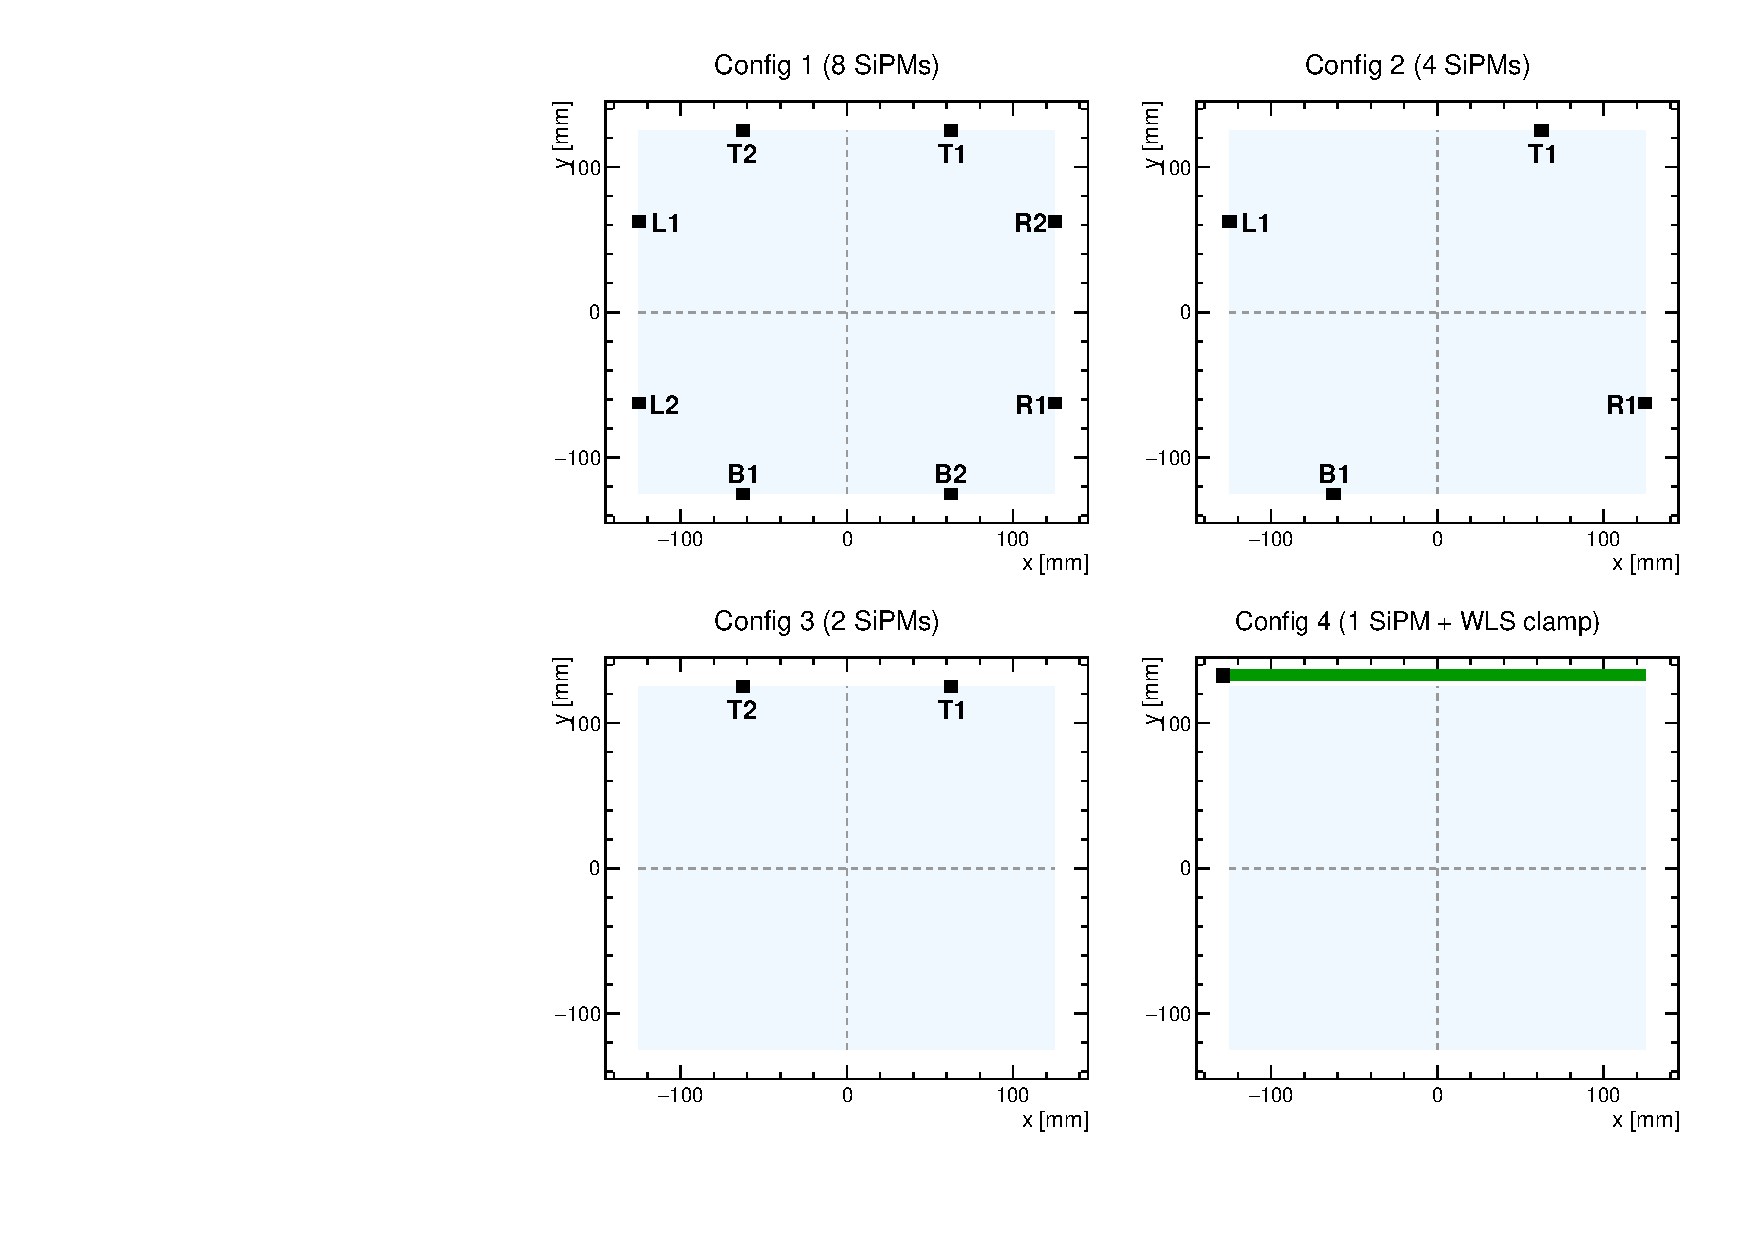
\includegraphics[width=0.72\textwidth]{fig1_layouts.pdf}
\caption{Plan view of the four layouts on the
\SI{250}{\milli\meter}$\times$\SI{250}{\milli\meter} plate. Black squares mark
the SiPMs (oversized for visibility); the dashed lines are the $x=0$ and $y=0$
axes. Config~1 uses eight sensors, config~2 four (one per face, at the
config-1 offsets), config~3 two on the top edge, and config~4 a single SiPM at
the left end of the WLS-fibre clamp on the top edge. The labels T/B/R/L denote
the four faces and the numerals the two offsets on each face.}
\label{fig:layouts}
\end{figure}

\subsection{Reflector treatments}
\label{sec:reflectors}

The four treatments are applied as logical skins on the non-instrumented
surfaces; the grease/SiPM patches override the skin locally through border
surfaces. Table~\ref{tab:surfaces} lists the parameters actually attached in the
code. The mapping is the heart of the model because it determines the
light-collection ordering.

\paragraph{Bare plate in a black holder.}
No skin is attached to the plate. The native polished scintillator--air boundary
($n=1.58$ to $1.0003$) is separated from the black holder by a real
\SI{1.2}{\milli\meter} air gap. Light below the critical angle
$\theta_c=\arcsin(1/1.58)=\SI{39.3}{\degree}$ refracts across the gap and is
absorbed by the holder, whose skin has $R=T=0$ and whose bulk absorption length
is \SI{1}{\micro\meter}. Light above $\theta_c$ is returned by TIR. The SiPMs
are still coupled through grease pads, so the plate is not isolated from the
read-out. This is the least constrained configuration: it assumes the plate is
everywhere decoupled from the holder. In configs~1--3 the black holder is built;
in config~4 the clamp replaces the holder on the instrumented face, so the
``bare'' label there means only that no reflector skin is applied.

\paragraph{TiO$_2$ paint.}
The plate is coated directly with a white diffuse paint, modelled as
\texttt{groundfrontpainted}: a random draw against $R(\lambda)$ returns the
photon with a Lambertian distribution and no specular or TIR component. The
reflectance rises from \num{0.955} in the ultraviolet to \num{0.983} near
\SI{470}{\nano\meter}. This is the physically correct description of a thick
scattering paint, but the absolute curve is a fitted white-paint
representative, not a measurement of EJ-510.

\paragraph{Aluminium foil with grease.}
The foil is modelled as \texttt{polishedbackpainted} with the backing index set
to the coupling grease ($n=1.46$). The scintillator--grease interface is a
Fresnel/TIR boundary with a wide critical angle,
\begin{equation*}
\theta_c=\arcsin(1.46/1.58)=\SI{67.5}{\degree},
\end{equation*}
so most light refracts into the grease and is returned by the foil as a pure
specular reflection. The reflectance is the
normal-incidence value of evaporated aluminium computed from the McPeak
$n,k$ data~\cite{McPeak2015}, \num{0.904}--\num{0.925}. Household foil is
rougher and oxidised, so this is an upper bound; the grease contact is idealised
as uniform.

\paragraph{High-gloss paper.}
The paper is wrapped with an air gap and modelled as
\texttt{polishedbackpainted} with the backing index set to air. The plate keeps
its full TIR cone and only the sub-critical fraction crosses the gap to the
paper, which returns it specularly with a fitted
$R(\lambda)\approx\num{0.900}$--\num{0.955}. The reference measurement reports
glossy paper and aluminium as the two brightest wrappers, which motivates
modelling glossy paper as a slightly lossy mirror rather than a diffuser. This
is a model choice: real photo paper has a diffuse component and its reflectance
was not measured independently.

\begin{table}[htbp]
\centering
\caption{Principal parameters of the scintillator, WLS fibre and SiPM adopted in
the simulation, compared with the values quoted in Ref.~\cite{Rao2025}. A dash
marks a quantity not reported or not modelled. The density and Birks constant
are taken from the \gfour{} NIST database and Ref.~\cite{Craun1970},
respectively, not from the UPS-92S data sheet.}
\label{tab:params}
\footnotesize
\begin{tabularx}{\textwidth}{@{}>{\raggedright\arraybackslash}p{0.27\textwidth} L L@{}}
\toprule
Parameter & Ref.~\cite{Rao2025} & This simulation \\
\midrule
\multicolumn{3}{@{}l}{\emph{Scintillator}}\\
Material & UPS-92S (AdvTECH UK) & PVT (\texttt{G4\_PLASTIC\_}\allowbreak\texttt{SC\_}\allowbreak\texttt{VINYLTOLUENE}) \\
Dimensions & $250\times250\times\SI{10}{\milli\meter}$ & $250\times250\times\SI{10}{\milli\meter}$ \\
Refractive index & 1.58 & 1.58 \\
Density & \SI{1.05}{\gram\per\cubic\centi\meter} & \SI{1.032}{\gram\per\cubic\centi\meter} \\
Light output & 50--60\% of anthracene & \SI{1.0e4}{\per\mega\electronvolt} \\
Emission peak & \SI{425}{\nano\meter} & \SI{425}{\nano\meter} \\
Bulk attenuation length & \SI{2000}{\milli\meter} & \SI{3.8}{\meter} (peak) \\
Decay / rise time & \SI{2.4}{\nano\second} / --- & \SI{2.1}{\nano\second} / \SI{0.9}{\nano\second} \\
Birks constant & --- & \SI{0.126}{\milli\meter\per\mega\electronvolt} \\
Surface finish & polished & polished \\
\midrule
\multicolumn{3}{@{}l}{\emph{WLS fibre (Kuraray Y-11(200))}}\\
Diameter & \SI{1.0}{\milli\meter} & \SI{1.0}{\milli\meter} \\
Cladding & multi-clad & PMMA ($n=1.49$) + fluoropolymer ($n=1.42$) \\
Core index & --- & 1.59 \\
Absorption / emission peak & \SI{430}{\nano\meter} / \SI{476}{\nano\meter} & \SI{430}{\nano\meter} / \SI{476}{\nano\meter} \\
WLS absorption length at \SI{430}{\nano\meter} & --- & \SI{1.0}{\milli\meter} \\
WLS decay time & --- & \SI{7}{\nano\second} (exponential) \\
Read-out & 4 fibres, one row, \SI{250}{\milli\meter} & 4 fibres, \SI{2.5}{\milli\meter} pitch $\to$ \SI{1.0}{\milli\meter} bundle pitch \\
Channel diameter & --- & \SI{1.1}{\milli\meter} (\SI{0.05}{\milli\meter} air annulus) \\
\midrule
\multicolumn{3}{@{}l}{\emph{SiPM (CEFLA ASD-NUV4S-P-40)}}\\
Active area & $4\times\SI{4}{\milli\meter\squared}$ & $4\times\SI{4}{\milli\meter\squared}$ \\
Cells & 9340 & --- \\
Peak sensitivity & \SI{420}{\nano\meter} & \SI{410}{\nano\meter} \\
PDE at peak & 43\% & 0.431 (digitized) \\
Epoxy index & 1.5115 & 1.55 \\
Coupling & BC-630 grease & \SI{0.1}{\milli\meter} grease ($n=1.46$) \\
\bottomrule
\end{tabularx}
\end{table}

\begin{table}[htbp]
\centering
\caption{\gfour{} optical-surface parameters for the four reflectors, as
attached in the code; type and finish names are hyphenated for space, the
identifiers use underscores. $R(\lambda)$ is tabulated on a shared ten-point
\SIrange{360}{650}{\nano\meter} grid and quoted as its range; a dash marks a
property that is neither set nor used. The bare plate carries no surface object
and uses the built-in \texttt{glisur}/\texttt{polished} default; the black holder
carries an absorbing skin.}
\label{tab:surfaces}
\footnotesize
\begin{tabularx}{\textwidth}{@{}>{\raggedright\arraybackslash}p{0.22\textwidth} C C C C@{}}
\toprule
 & \textbf{Bare} & \textbf{TiO$_2$} & \textbf{Al foil} & \textbf{Glossy} \\
\midrule
Contact & \SI{1.2}{\milli\meter} air gap & direct & grease film & air gap \\
Surface object & none & skin & skin & skin \\
Type & dielectric--dielectric & dielectric--dielectric & dielectric--dielectric & dielectric--dielectric \\
Model & glisur & unified & unified & unified \\
Finish & polished & ground-front-painted & polished-back-painted & polished-back-painted \\
$\sigma_\alpha$ & --- & 0.10 rad & 0 & 0 \\
$R(\lambda)$ & --- & 0.955--0.983 & 0.904--0.925 & 0.900--0.955 \\
Backing index & --- & --- & 1.46 & 1.0003 \\
$f_{ss}$ / $f_{sl}$ / $f_{bs}$ & --- & 0 / 0 / 0 & 1 / 0 / 0 & 1 / 0 / 0 \\
TIR & $\theta>\SI{39.3}{\degree}$ & no & $\theta>\SI{67.5}{\degree}$ & $\theta>\SI{39.3}{\degree}$ \\
\bottomrule
\end{tabularx}
\end{table}

\subsection{WLS-fibre clamp (config 4)}
\label{sec:wls}

Four \SI{1.0}{\milli\meter}-diameter Kuraray Y-11(200) multi-clad
fibres~\cite{KurarayPSF,Alekseev2022} run the full \SI{250}{\milli\meter} length
of one narrow face in a single row. In the straight section the centre-to-centre
pitch is \SI{2.5}{\milli\meter}, so a solid web of clamp material separates the
milled \SI{1.1}{\milli\meter} channels. Over the last \SI{41}{\milli\meter}
(\SI{39}{\milli\meter} ramp plus a \SI{2}{\milli\meter} stub) the fibres
converge to a touching bundle with \SI{1.0}{\milli\meter} pitch that presents all
four ends to one \SI{4}{\milli\meter}$\times$\SI{4}{\milli\meter} SiPM; the far ends are
closed by aluminium mirror caps. Each fibre is a Y-11 core ($n=1.59$) inside a
PMMA inner cladding ($n=1.49$) inside a fluoropolymer outer sheath ($n=1.42$).
The production solid is an analytic, mitered set of \texttt{G4CutTubs} legs, one
per straight segment of the bent centreline, placed so adjoining legs meet at
exact miter planes; this avoids the degenerate facets of the earlier tessellated
variant. A \SI{0.10}{\milli\meter} grease film couples the plate face to the
clamp, and each fibre protrudes \SI{0.05}{\milli\meter} into that film. The
\SI{0.05}{\milli\meter} air annulus between fibre and channel is deliberate: the
fibre must not touch the $n=1.55$ clamp, and the low-index sheath needs the
clearance to guide light. The clamp is white 3D-printed plastic, modelled as a
Lambertian reflector with \SI{85}{\percent} reflectivity on every face. A skin
on the mirror caps ensures that light travelling in the core, not only in the
cladding, is turned around at the far end. WLS re-emission uses the digitized
Y-11 emission spectrum with an exponential delay of \SI{7}{\nano\second}; the
\texttt{G4OpWLS} process is enabled automatically when the geometry is built.

\begin{figure}[htbp]
\centering
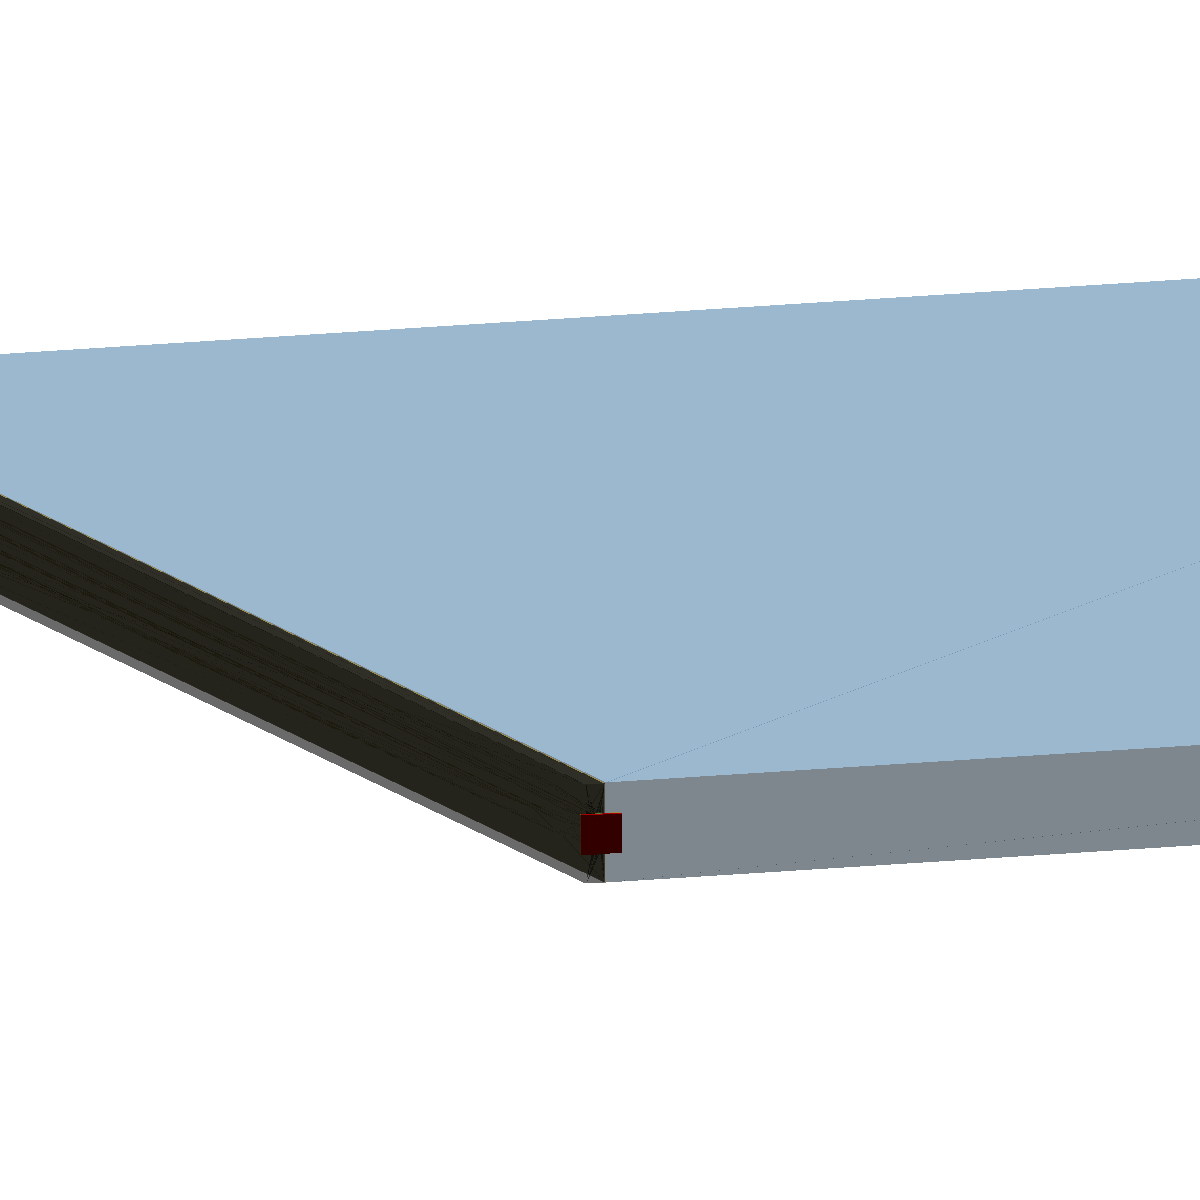
\includegraphics[width=0.72\textwidth]{fig3_wls_geometry.png}
\caption{Oblique render of the config-4 assembly: the \SI{250}{\milli\meter}
plate with the WLS-fibre clamp on one narrow face and the single read-out SiPM
at the end of the converged bundle. The four fibres run the full plate length.
The render is geometry-only (no beam) and uses the tessellated visualisation
preset; the production geometry uses the analytic mitered solid described in
the text.}
\label{fig:wls}
\end{figure}

\subsection{Optical inputs and boundary physics}
\label{sec:physics}

Optical photons are transported by the standard \gfour{} optical module, with
scintillation, \v{C}erenkov, bulk absorption, Rayleigh scattering and boundary
processes active. Mie scattering is disabled; \texttt{G4OpWLS} is enabled only
for config~4. Figure~\ref{fig:inputs} shows the spectral tables actually fed to
\gfour: the scintillator emission and bulk attenuation, the Y-11 absorption and
re-emission, and the SiPM PDE. The Y-11 absorption peaks at \SI{430}{\nano\meter}
and is effectively transparent red-ward of \SI{500}{\nano\meter}; the emission
peaks at \SI{476}{\nano\meter}. The emission table is zero red-ward of the
absorption onset ($\lambda\ge\SI{488}{\nano\meter}$), but it extends to shorter
wavelengths, so a small high-energy tail overlaps the absorption band and mild
self-absorption is present by construction.

The boundary process selects a surface from a \texttt{G4LogicalBorderSurface}
first and a \texttt{G4LogicalSkinSurface} second; if neither exists it falls back
to a lossless TIR default. A valid \texttt{RINDEX} is required on medium~1
always and on medium~2 for a \texttt{polished}/\texttt{ground}
\texttt{dielectric\_dielectric} boundary; \texttt{*backpainted} finishes read the
backing index from the surface. A missing index produces a silent
\texttt{NoRINDEX} kill, so every material and backpainted surface carries an
explicit table. This is also why the far-end mirror needs a skin: the metal cap
has no \texttt{RINDEX}, and the uncovered core-to-cap crossing would otherwise be
lost.

For the unified model, the reflection weights are
\texttt{SPECULARSPIKECONSTANT} ($f_{ss}$), \texttt{SPECULARLOBECONSTANT}
($f_{sl}$) and \texttt{BACKSCATTERCONSTANT} ($f_{bs}$), together with
\texttt{REFLECTIVITY}. The finish selects the code path:
\texttt{groundfrontpainted} is a pure Lambertian draw with no TIR;
\texttt{polishedbackpainted} is a Fresnel/TIR dielectric boundary followed by a
backing reflection; and the bare plate uses the default polished
dielectric--dielectric boundary. Photodetection is delegated to the
\texttt{dielectric\_metal} grease/SiPM boundary. In \texttt{DielectricMetal()},
an absorbed photon is classified as \texttt{Detection} only when a uniform draw
is below the tabulated PDE; when the boundary-invoke-SD flag is set, the
sensitive detector is called only for that outcome. The sensitive detector
therefore books one hit per genuine photoelectron and kills the photon; there is
no separate random draw in user code.

\begin{figure}[htbp]
\centering
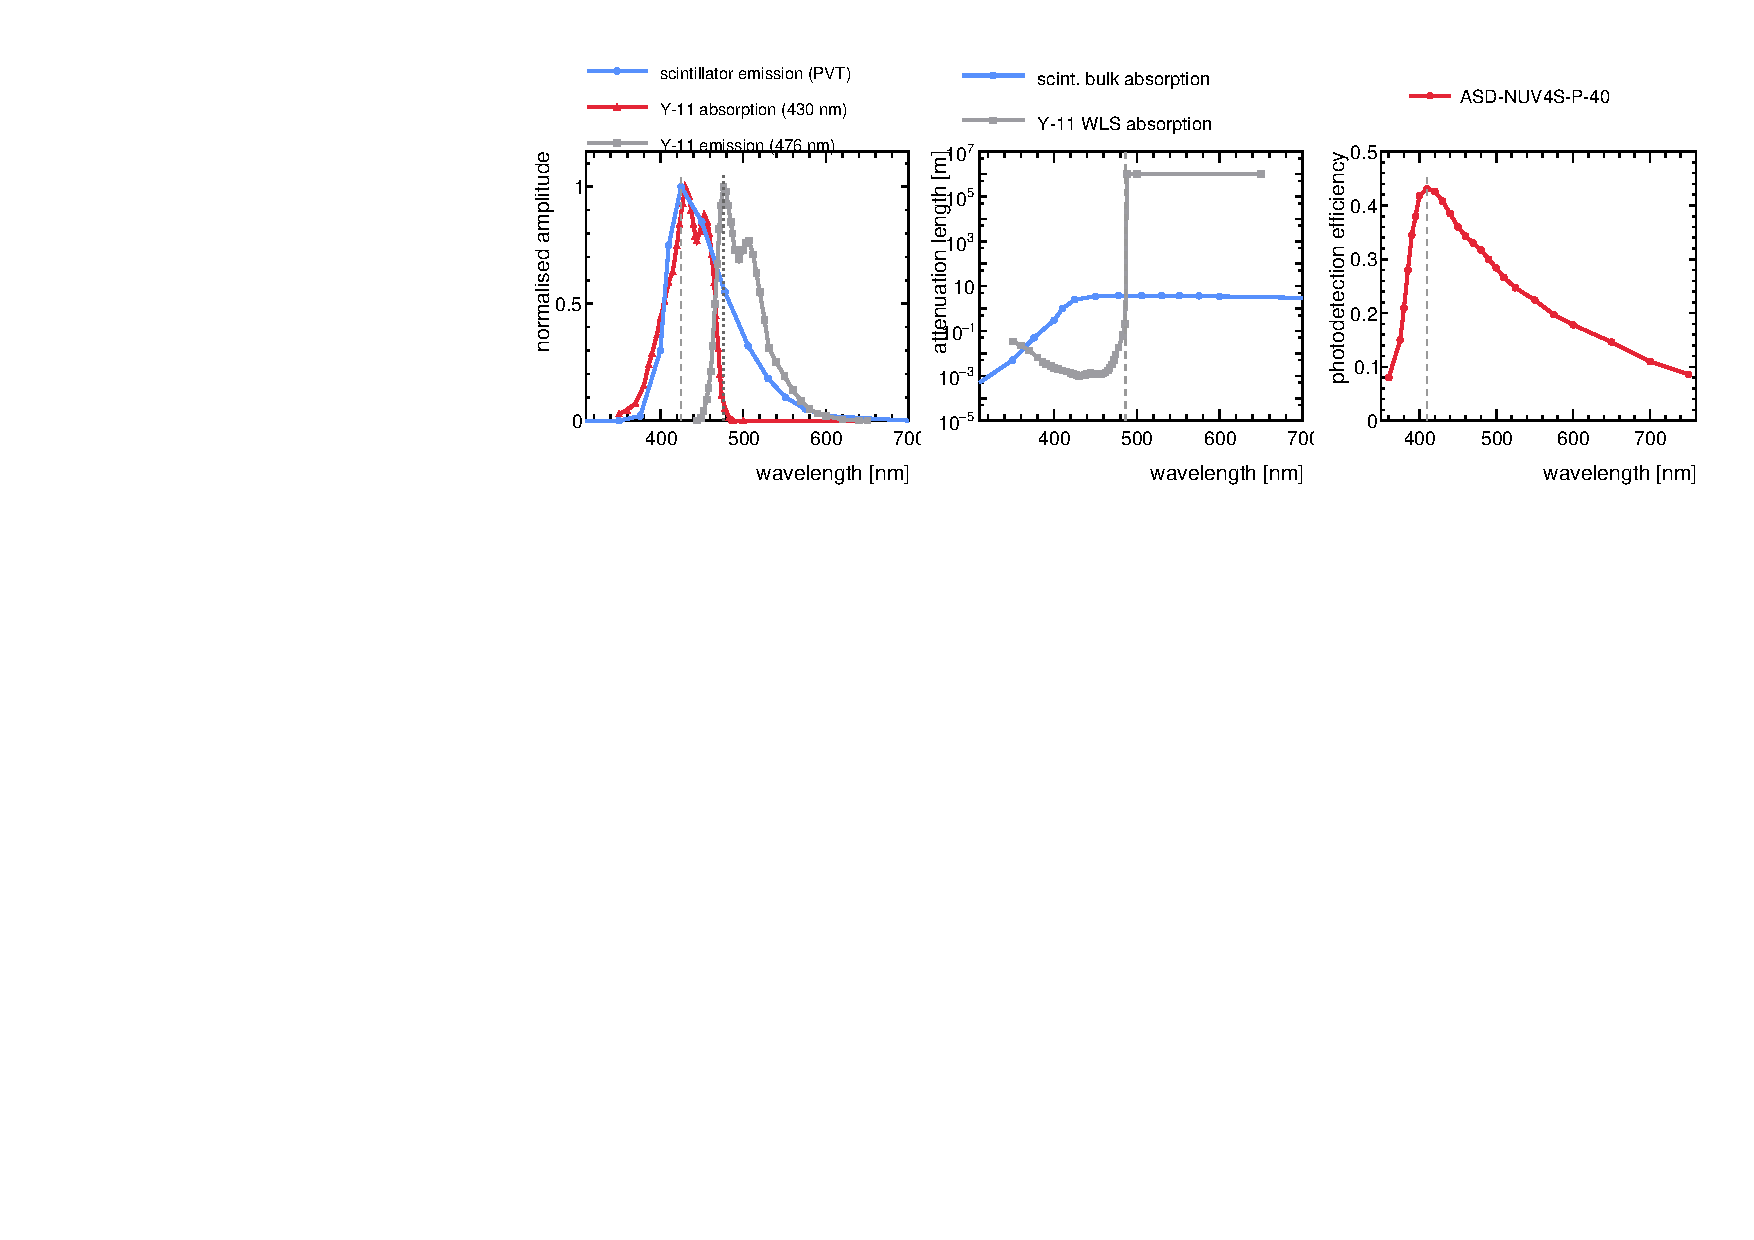
\includegraphics[width=\textwidth]{fig2_optical_inputs.pdf}
\caption{Optical property tables used by the simulation. Left: normalized
scintillator emission, Y-11 absorption and Y-11 re-emission. Middle:
attenuation lengths on a logarithmic scale, including the scintillator bulk
curve and the fibre WLS absorption with \SI{1.0}{\milli\meter} at the
\SI{430}{\nano\meter} peak. Right: digitized SiPM PDE, peaking at \num{0.431}
near \SI{410}{\nano\meter}. Markers are the tabulated points and segments are
the linear interpolation used by \gfour.}
\label{fig:inputs}
\end{figure}

\section{Simulation campaign and observables}
\label{sec:method}

\subsection{Beam patches and efficiency definition}

The primary source is a vertical \SI{4}{\giga\electronvolt} $\mu^-$ beam with a
\SI{50}{\milli\meter} square profile. The
beam centre is placed at three positions in the report frame,
\[
\text{centre}=(0,0),\qquad
\text{edge}=(0,-100),\qquad
\text{corner}=(100,-100)\ \si{\milli\meter},
\]
which correspond to slab-local positions $(0,0)$, $(100,0)$ and $(100,100)$;
the illuminated regions are $[-25,25]^2$,
$[-25,25]\times[-125,-75]$ and $[75,125]\times[-125,-75]$. Each patch has the
same area and lies fully on the plate, so the produced-photon denominators are
equal. The edge and corner patches are on the bottom edge, opposite the
instrumented top face of configs~3 and~4, matching the reference layout. Each
(config, wrapper, patch) combination is run for \num{2500} events, giving
$4\times4\times3=48$ files and \num{120000} events. Whole-plate runs use a
\SI{250}{\milli\meter}$\times$\SI{250}{\milli\meter} GPS plane and \num{25000}
events per (config, wrapper), giving \num{400000} events. The total is
\num{520000} events, or about $1.0\times10^{10}$ tracked optical photons.

The collection efficiency for a set $\mathcal{S}$ of SiPMs is
\begin{equation}
\eps=\frac{\sum_e\sum_{s\in\mathcal{S}}\pe^{(e,s)}}{\sum_e\ngam^{(e)}},
\label{eq:eff}
\end{equation}
where $\pe^{(e,s)}$ is the number of photoelectrons in SiPM $s$ in event $e$ and
$\ngam^{(e)}$ is the number of optical photons produced in the slab (scintillation
plus \v{C}erenkov). The numerator and denominator are summed over events, so
$\eps$ is a ratio of totals, not a mean of per-event ratios. For the matrix, the
sum runs over all SiPMs of the layout and over the events of one patch. For the
whole-plate run, it runs over all events and yields the plate-averaged
efficiency. Statistical uncertainties are computed from the event-to-event
variance of the numerator at fixed denominator (delta method) and cross-checked
with Poisson errors on the photoelectron count; they are quoted in the tables.
Ref.~\cite{Rao2025} quotes a thresholded muon detection efficiency rather than a
raw photon-collection efficiency, so the comparison below is restricted to
orderings and relative scaling; the absolute \eps{} values are not directly
comparable.

The sensitive detector writes one row per (event, SiPM), including
zero-detection rows, so the sample is unbiased in the muon entry position. Each
row carries the entry position, the event's produced-photon count, the detected
count, the first arrival time, the mean and RMS detected wavelength, and
variable-length lists of the individual photoelectron arrival times,
wavelengths and creating processes (1 = \texttt{OpWLS}, 2 = scintillation,
3 = \v{C}erenkov). This allows the efficiency, spectra, timing and process mix
to be reconstructed offline at any binning.

\subsection{Whole-plate maps and uniformity}

The whole-plate events are binned by the primary muon's first-entry position in
$5\times\SI{5}{\milli\meter}$ cells, giving the field
\[
\eps(x,y)=
\frac{\sum_{e:(x_e,y_e)\in\mathrm{cell}}\sum_{s\in\mathcal{S}}\pe^{(e,s)}}
     {\sum_{e:(x_e,y_e)\in\mathrm{cell}}\ngam^{(e)}}.
\]
A purely radial contrast is not used: the layouts have no continuous rotational
symmetry and the plate is square, so a radial average would mix different
azimuths and, beyond the inscribed circle, sample only the corner wedges. The
uniformity is instead quantified on the plane by the normalized map
$\eps/\langle\eps\rangle$ and by the two-dimensional contrast
\begin{equation}
\ktwo=\frac{\max_{\mathrm{cell}}\eps}{\min_{\mathrm{cell}}\eps},
\end{equation}
evaluated on a $5\times5$ grid of \SI{50}{\milli\meter} cells. The coarser grid
is used because the \SI{5}{\milli\meter} cells are too sparse for a stable
max/min; $\ktwo$ is therefore a robust dynamic range, smaller than the raw
peak-to-trough range of the fine maps.

\section{Results}
\label{sec:results}

\subsection{Photon yield and photoelectron spectra}

Figure~\ref{fig:yieldpe} shows the per-event produced-photon yield and the
detected photoelectron count for config~1 at the centre patch. The mean yield is
essentially independent of the wrapper, about \num{1.9e4} photons per event, as
it must be: the wrapper changes transport, not production. The small spread
reflects the muon path-length distribution. The photoelectron spectra, in
contrast, depend strongly on the wrapper. At the config-1 centre the mean runs
from \num{124} pe/event for TiO$_2$ and \num{198} for aluminium to \num{305} for
the air-gap bare plate and \num{517} for glossy paper. The bare curve is not a
near-zero peak but a broad distribution comparable to the reflective wrappers,
the direct signature of near-lossless TIR transport. With a PDE of about
\num{0.4} and the geometric acceptance of a side-mounted sensor, a collection
efficiency of a few percent is expected; the best wrapper reaches
$517/1.9\times10^{4}\approx\SI{2.7}{\percent}$.

\begin{figure}[htbp]
\centering
\begin{subfigure}{0.49\textwidth}
  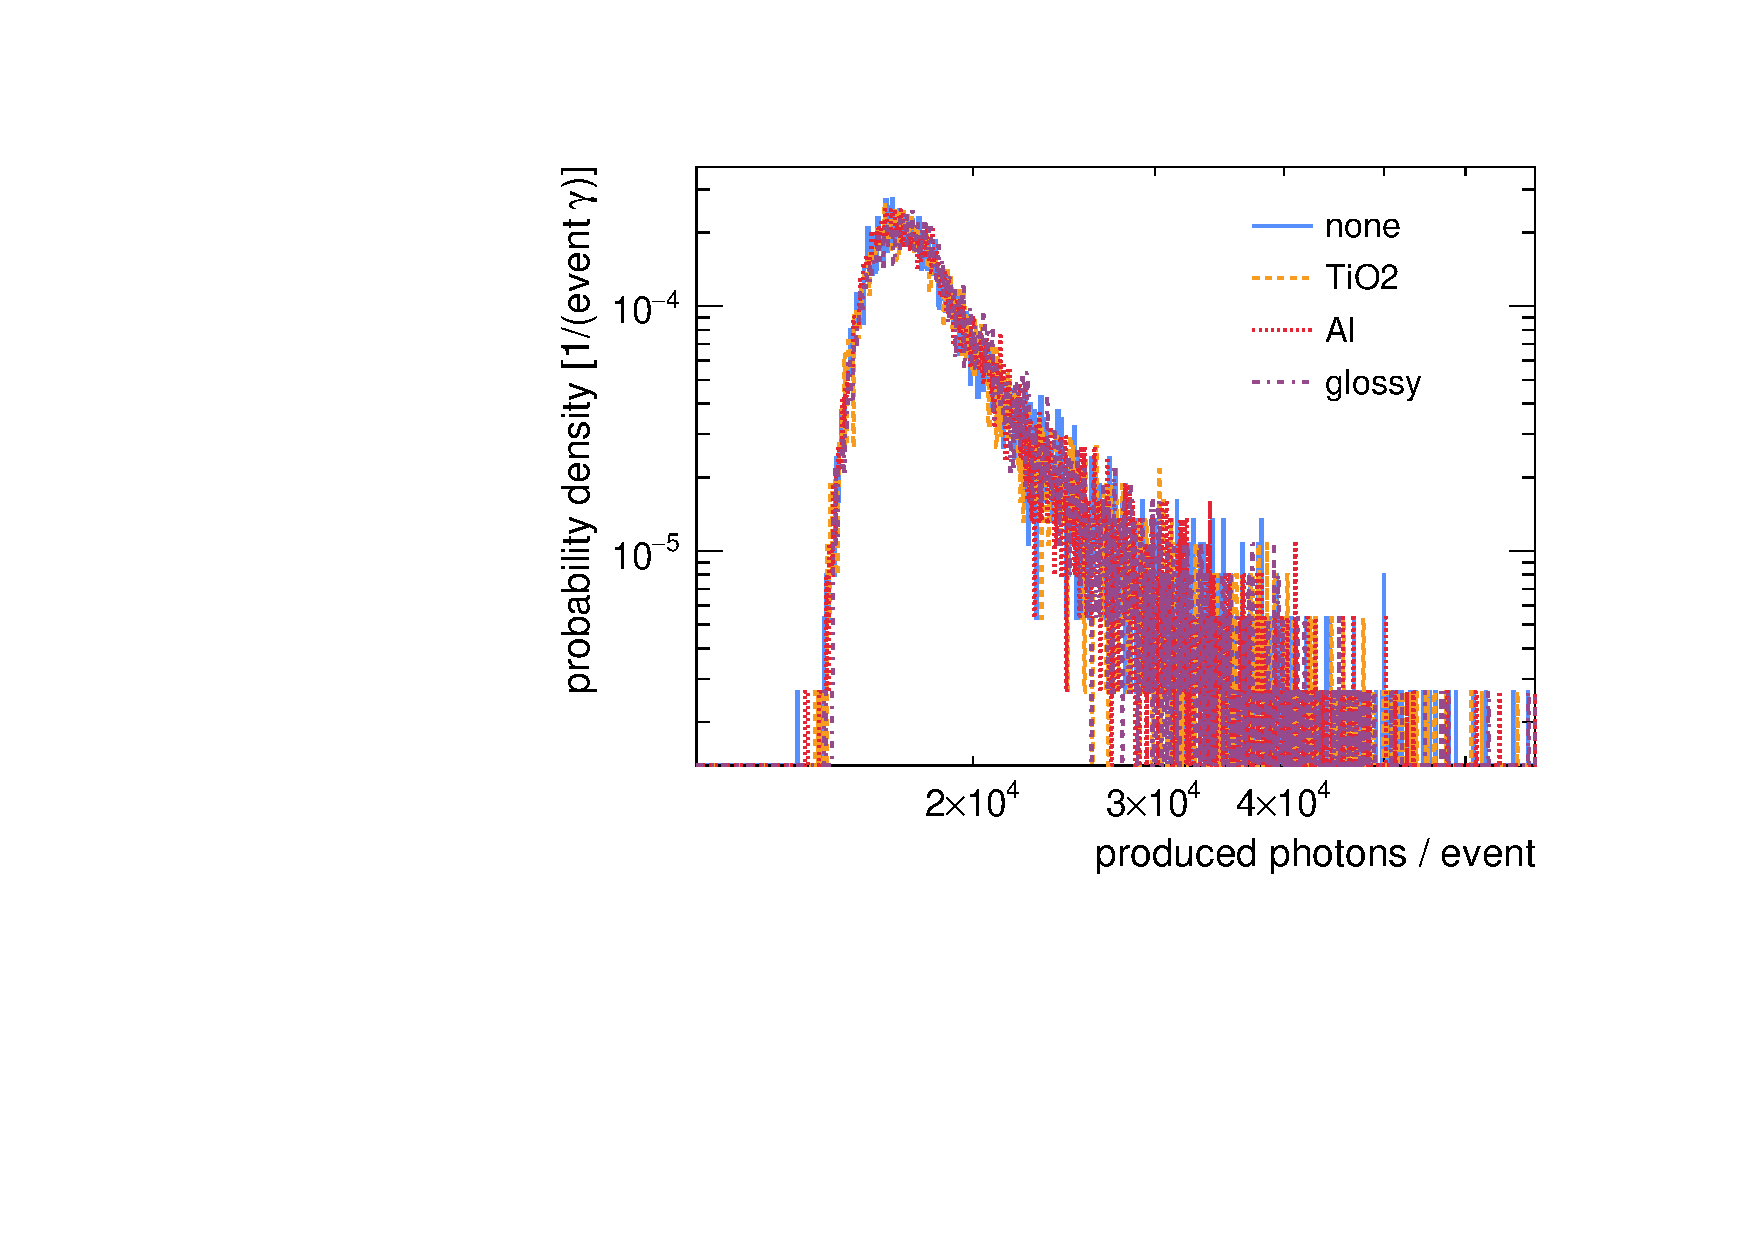
\includegraphics[width=\textwidth]{fig4a_yield.pdf}
  \caption{Produced photons per event.}
\end{subfigure}\hfill
\begin{subfigure}{0.49\textwidth}
  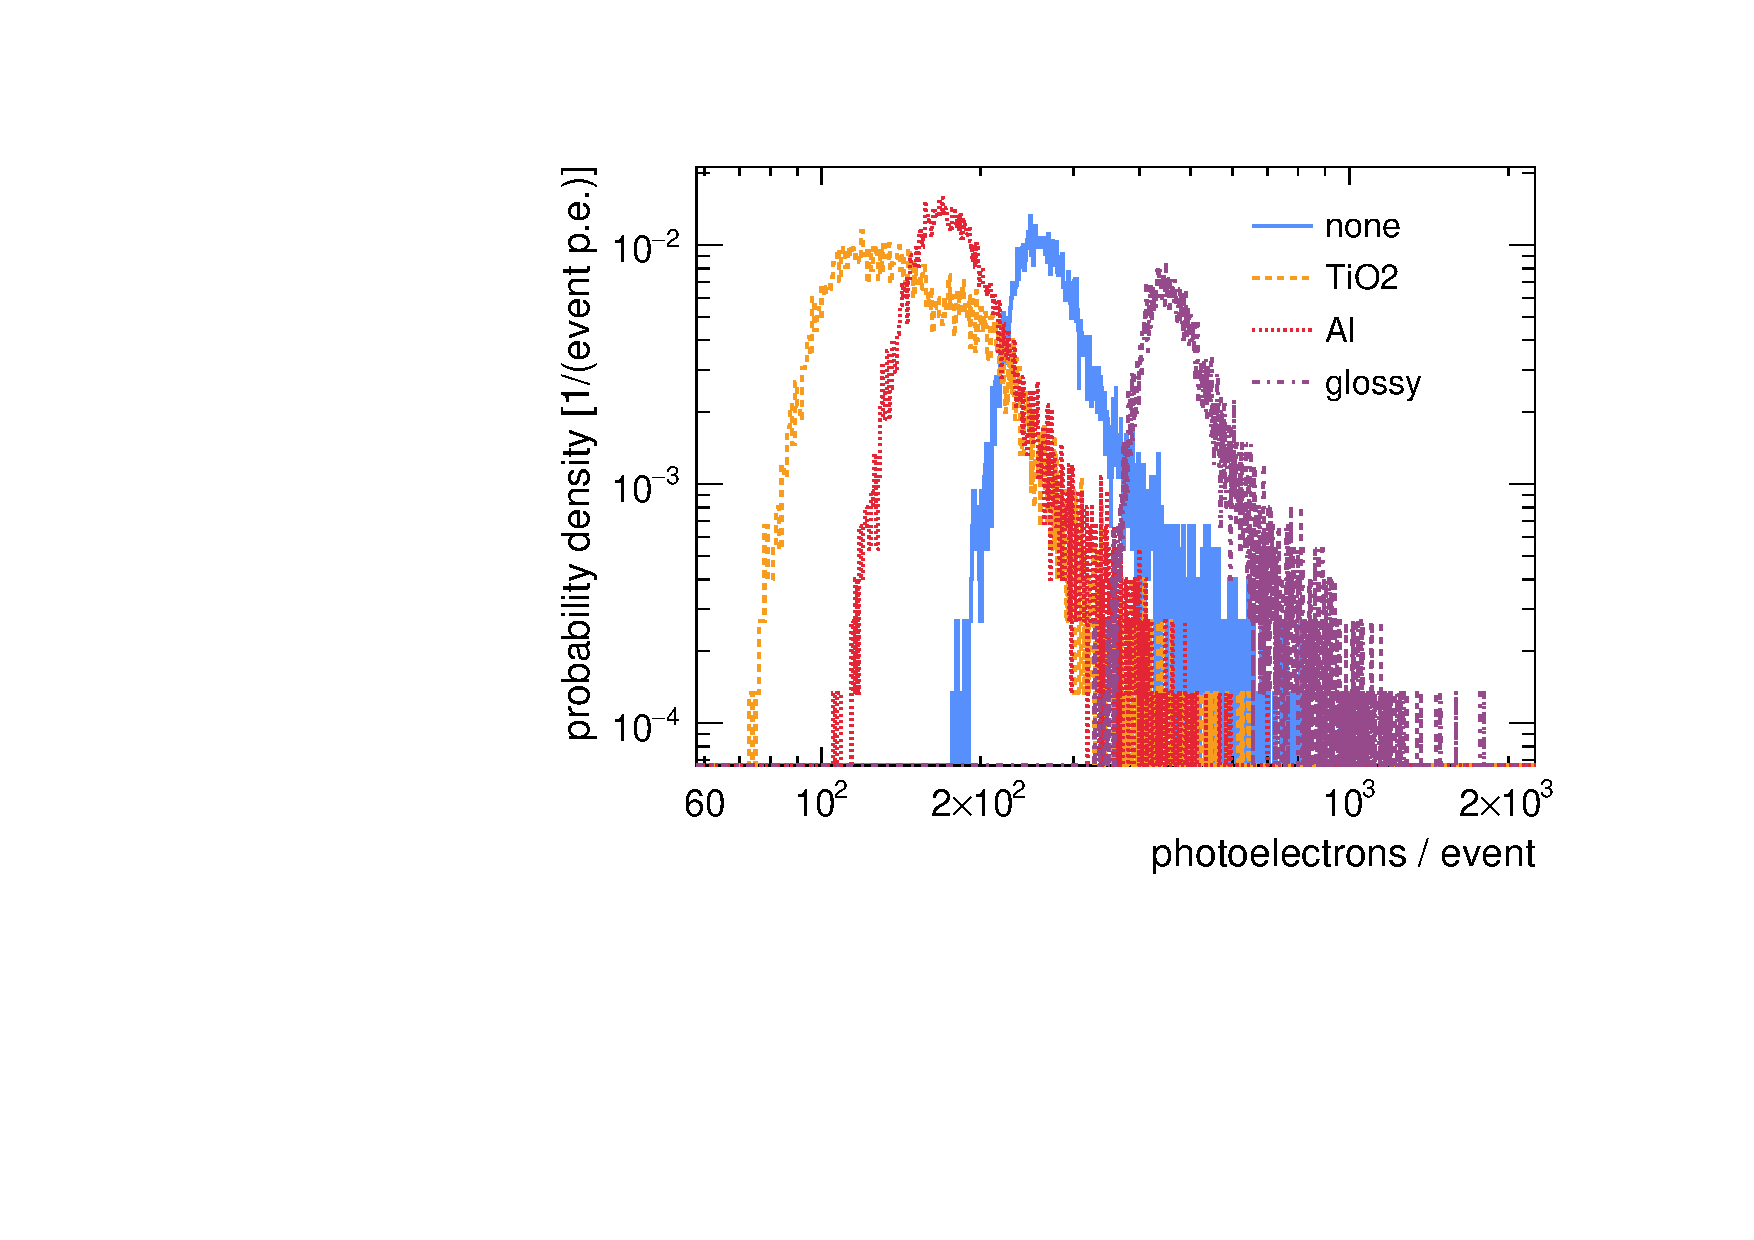
\includegraphics[width=\textwidth]{fig4b_detected.pdf}
  \caption{Detected photoelectrons per event.}
\end{subfigure}
\caption{Per-event distributions for config~1 at the centre patch, plotted as
probability densities with logarithmic axes. The production yield (left) is
wrapper-independent; the detected count (right) depends strongly on the
wrapper. The air-gap bare plate is close to the reflective wrappers, not to
zero.}
\label{fig:yieldpe}
\end{figure}

\subsection{Wrapper ordering and layout scaling}

Figure~\ref{fig:ordering} shows the plate-averaged efficiency for all
(config, wrapper) pairs, and Table~\ref{tab:eff} lists the numbers. Glossy paper
is the brightest wrapper in every layout. In the three direct-coupled layouts
the ordering is
\[
\text{TiO}_2 < \text{Al} < \text{bare} < \text{glossy},
\]
with the bare plate second, not last. In the WLS layout the order changes to
\[
\text{Al} < \text{TiO}_2 < \text{bare} < \text{glossy},
\]
so the aluminium foil becomes the weakest wrapper. The spread from weakest to
brightest within a layout is a factor of \num{2.3}--\num{2.9}. The efficiency
scales roughly with the photosensitive area: config~1 is highest, config~2 is
about \num{1.9} times lower, config~3 another factor of about \num{1.9}, and
config~4 a further factor of \num{2.1}--\num{2.5}. The WLS layout collects the
fewest photoelectrons because only the fraction of light reaching the fibre face
is shifted and guided to the single sensor.

The physical interpretation is straightforward. For the bare plate, the
critical angle is \SI{39.3}{\degree}, so most of the solid angle is trapped by
TIR; only the escape cone is lost to the holder, apart from the instrumented
pads. For glossy paper, the air gap
preserves the same TIR cone and the paper returns part of the escape cone
specularly, so glossy is brighter than bare. For aluminium with grease, the
critical angle widens to \SI{67.5}{\degree}: a much larger fraction enters the
grease and is reflected by the foil with $R\approx\num{0.9}$, and the repeated
Fresnel and reflection losses make it dimmer than the bare TIR guide. For
TiO$_2$, there is no TIR at all; every photon is either diffusely reflected with
$R\approx\num{0.96}$ or absorbed, and the random walk loses photons at every
bounce. The WLS layout changes the balance because the fibres accept only a
small solid angle at the clamp face, and the aluminium foil's high-angle
transmission is no longer an advantage.

\begin{figure}[htbp]
\centering
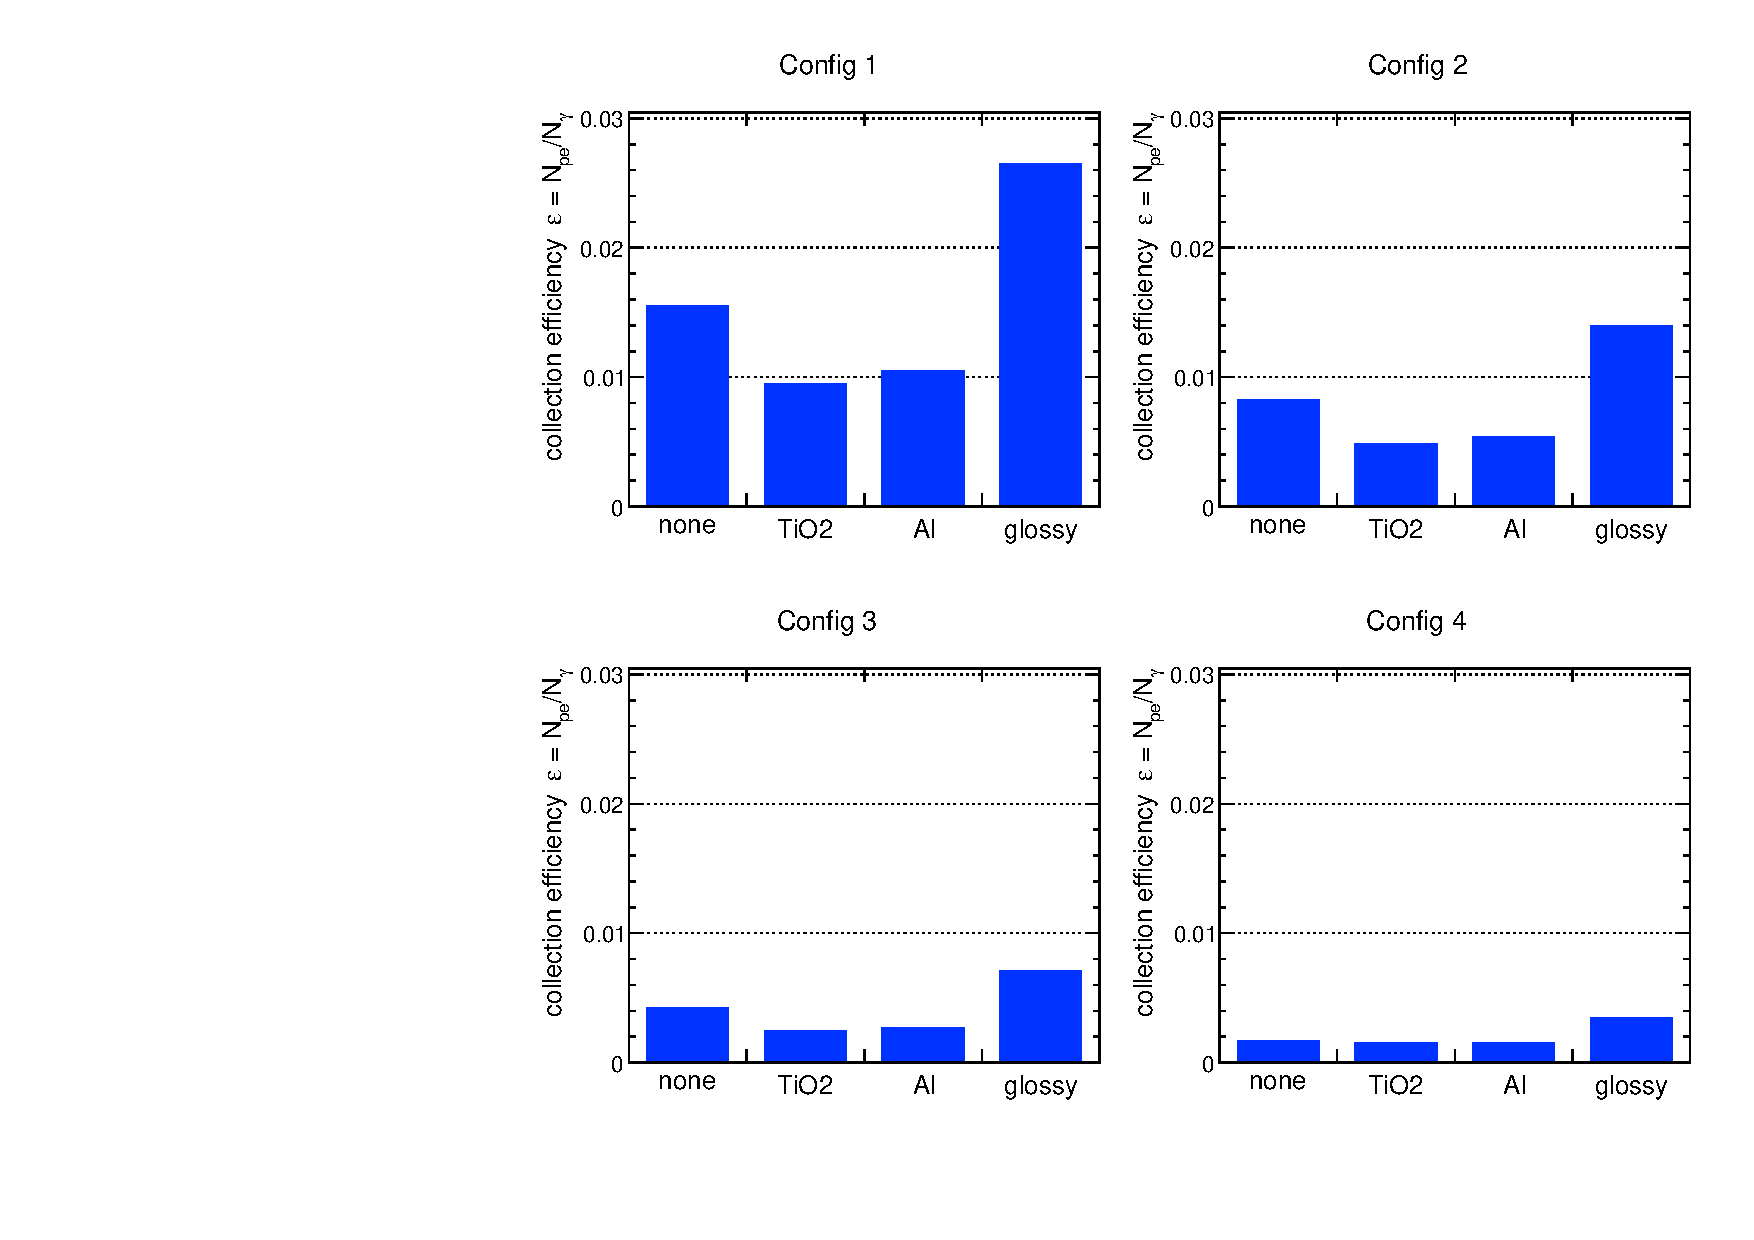
\includegraphics[width=0.88\textwidth]{fig6_eff_bars.pdf}
\caption{Plate-averaged collection efficiency for the four wrappers and four
layouts, from the uniform whole-plate irradiation (\num{25000} events per
panel). Glossy paper is brightest everywhere; the air-gap bare plate is second
in the direct-coupled layouts and third in the WLS layout, where aluminium is
weakest.}
\label{fig:ordering}
\end{figure}

\begin{table}[htbp]
\centering
\caption{Plate-averaged collection efficiency (all SiPMs, uniform whole-plate
irradiation), in units of $10^{-3}$. The number in parentheses is the
statistical uncertainty in the last digits.}
\label{tab:eff}
\small
\begin{tabular}{@{}lcccc@{}}
\toprule
Layout & Bare & TiO$_2$ & Al & Glossy \\
\midrule
Config 1 (8 SiPMs)     & 15.542(12) & 9.5318(22) & 10.4932(12) & 26.4795(12) \\
Config 2 (4 SiPMs)     & 8.2579(9)  & 4.8596(16) & 5.4057(9)   & 13.9865(9)  \\
Config 3 (2 SiPMs)     & 4.2438(6)  & 2.4552(15) & 2.7254(7)   & 7.1564(7)   \\
Config 4 (1 SiPM, WLS) & 1.7265(2)  & 1.5891(8)  & 1.5145(2)   & 3.4698(3)   \\
\bottomrule
\end{tabular}
\end{table}

\subsection{Position dependence}

Figure~\ref{fig:positions} groups the three beam patches by layout, and
Table~\ref{tab:positions} lists the config-1 values with uncertainties. The bare
plate and the specular wrappers are nearly flat: for glossy, aluminium and bare
the efficiency varies by at most \SI{6}{\percent} across the three patches in
every layout. Only TiO$_2$ shows a clear position dependence, with a factor of
about \num{1.75} in config~1. In the four-sided layouts the TiO$_2$ response is
corner $>$ edge $>$ centre; in the single-sided layouts it is centre $>$ edge
$\approx$ corner. The sign follows the distance from the illuminated patch to
the instrumented face, not a simple radius: in the single-sided layouts the
centre patch is closer to the sensors than the edge and corner patches, which
lie on the opposite side.

The near-flatness of the bare and specular responses is the signature of a
well-mixed cavity: after a few bounces the light no longer remembers where the
muon crossed, so the sensor coverage, not the irradiation point, sets the
collection. The diffuse paint retains a memory of the source position because
each Lambertian bounce randomizes the direction and the light is gradually
absorbed; the response is highest where the painted walls can return light
efficiently to the sensors.

\begin{figure}[htbp]
\centering
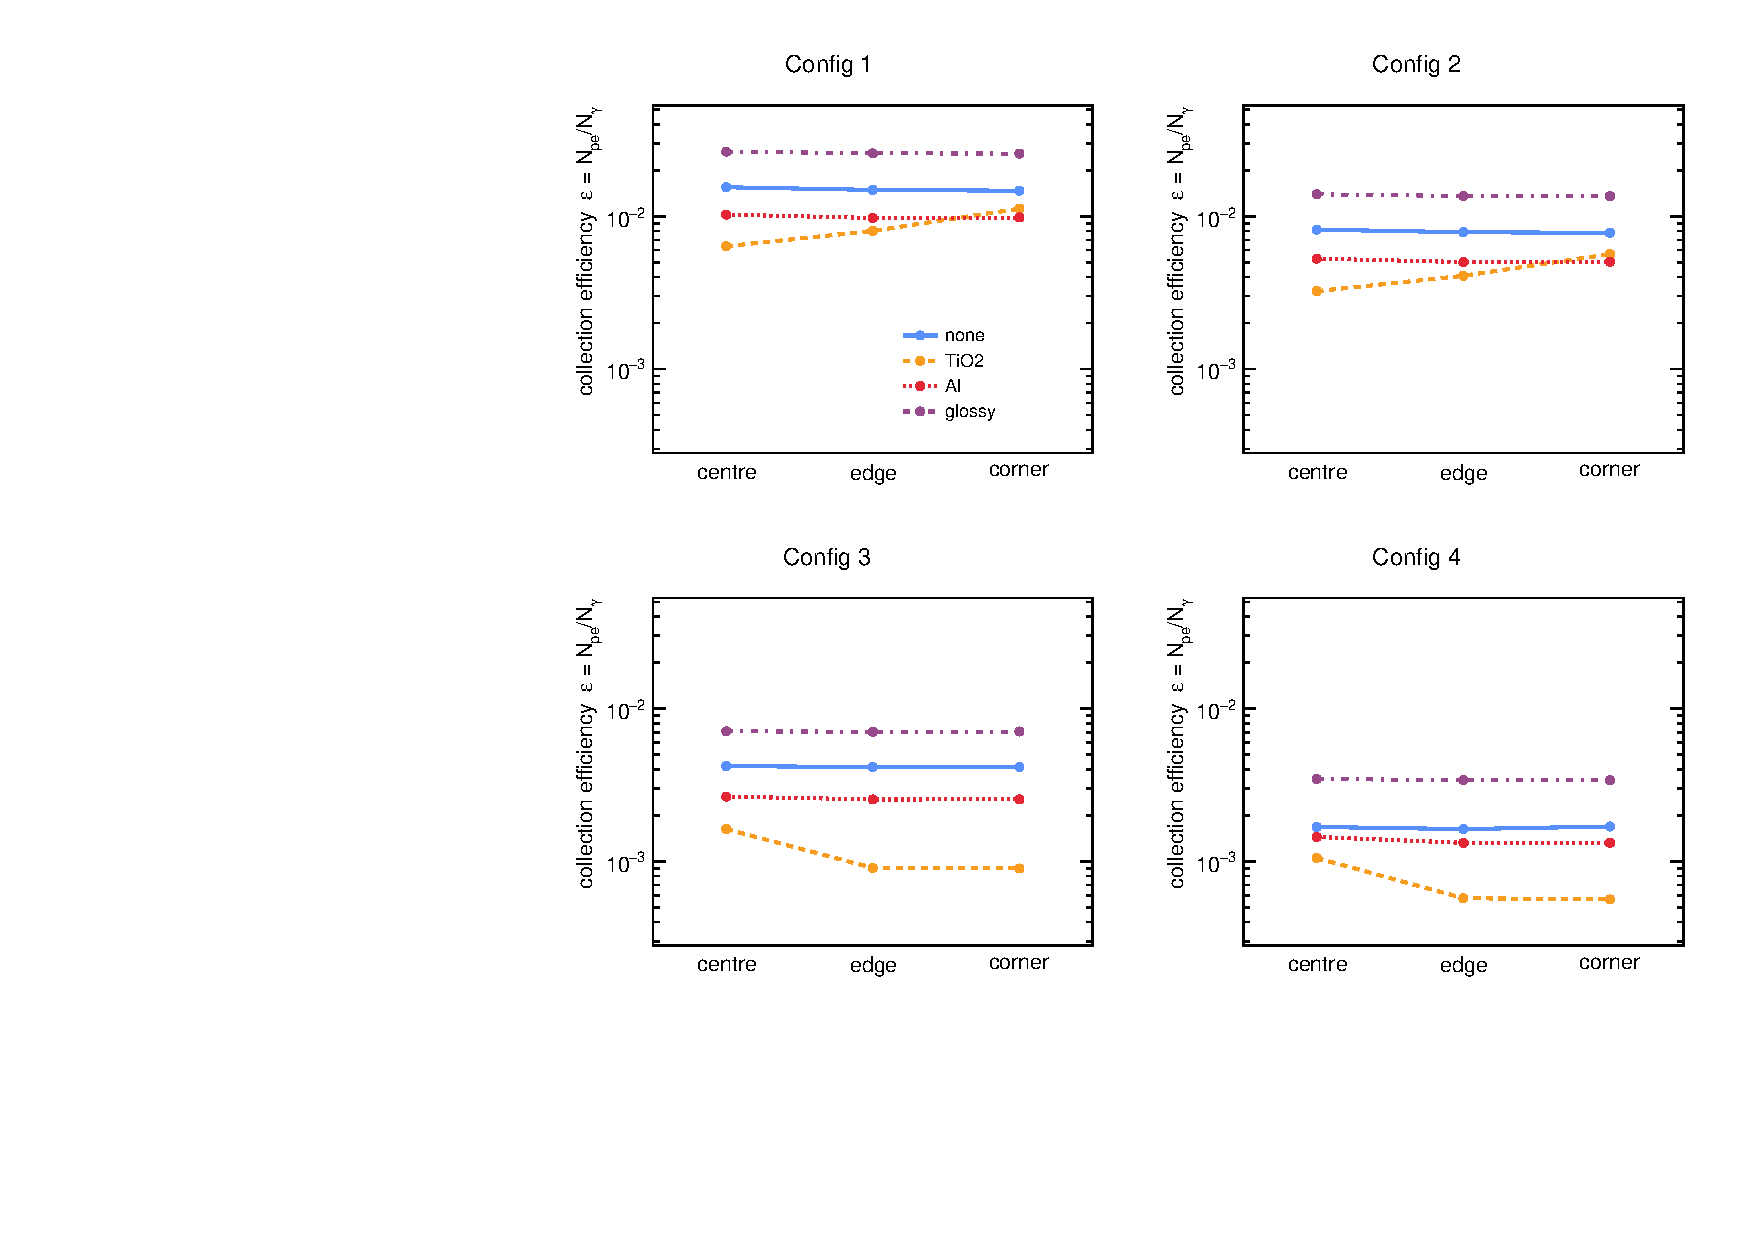
\includegraphics[width=\textwidth]{fig5_positions.pdf}
\caption{Collection efficiency at the three beam patches, one panel per layout,
with the four wrapper curves (logarithmic ordinate). All patches have equal area
and lie fully on the plate. The bare and specular wrappers are nearly flat;
TiO$_2$ is the only wrapper with a clear position dependence, and its sign
depends on whether the layout is four-sided or single-sided.}
\label{fig:positions}
\end{figure}

\begin{table}[htbp]
\centering
\caption{Position dependence of the collection efficiency for config~1 (all
SiPMs). Each patch is \SI{50}{\milli\meter}$\times$\SI{50}{\milli\meter} and
lies fully on the plate. The number in parentheses is the statistical
uncertainty in the last digits.}
\label{tab:positions}
\small
\begin{tabular}{@{}lccc@{}}
\toprule
Wrapper & Centre & Edge & Corner \\
\midrule
Bare   & $1.5485(18)\times10^{-2}$ & $1.4880(19)\times10^{-2}$ & $1.4695(26)\times10^{-2}$ \\
TiO$_2$& $6.3687(12)\times10^{-3}$ & $8.0219(15)\times10^{-3}$ & $1.12188(27)\times10^{-2}$ \\
Al     & $1.02503(15)\times10^{-2}$ & $9.7520(16)\times10^{-3}$ & $9.8319(24)\times10^{-3}$ \\
Glossy & $2.64660(24)\times10^{-2}$ & $2.58179(25)\times10^{-2}$ & $2.56926(30)\times10^{-2}$ \\
\bottomrule
\end{tabular}
\end{table}

\subsection{Whole-plate maps and uniformity}

Figure~\ref{fig:maps} shows the full-plate efficiency maps for config~1. The
bare map is nearly flat: the mean within $r<\SI{60}{\milli\meter}$
($1.54\times10^{-2}$) differs from the outer region ($1.56\times10^{-2}$) by
under \SI{2}{\percent}. Aluminium and glossy are also flat; TiO$_2$ is the only
wrapper with a clear gradient, and it runs the other way, with the centre
($6.7\times10^{-3}$) dimmer than the edge and corner
($1.02\times10^{-2}$), a factor of about \num{1.5}. The same pattern repeats in
the other layouts: the bare and specular responses remain nearly flat, while
TiO$_2$ darkens where the source is far from the instrumented face.

The uniformity ranking is the same in every layout,
\[
\text{TiO}_2 > \text{Al} > \text{bare} \gtrsim \text{glossy},
\]
as quantified by $\ktwo$ in Table~\ref{tab:kappa}. The diffuse paint is the
least uniform wrapper, with $\ktwo$ growing from \num{1.90} in config~1 to
\num{8.46} in config~3; the bare plate stays at \num{1.13}--\num{1.47} and the
specular wrappers at \num{1.07}--\num{1.79}. For the bare and specular wrappers
a muon crossing anywhere on the plate is collected within about a factor of two
of the most favourable point. For TiO$_2$ in the single-sided layouts the
corner-to-centre penalty approaches an order of magnitude. This is the strongest
argument against a diffuse wrapper when position uniformity matters.

\begin{figure}[htbp]
\centering
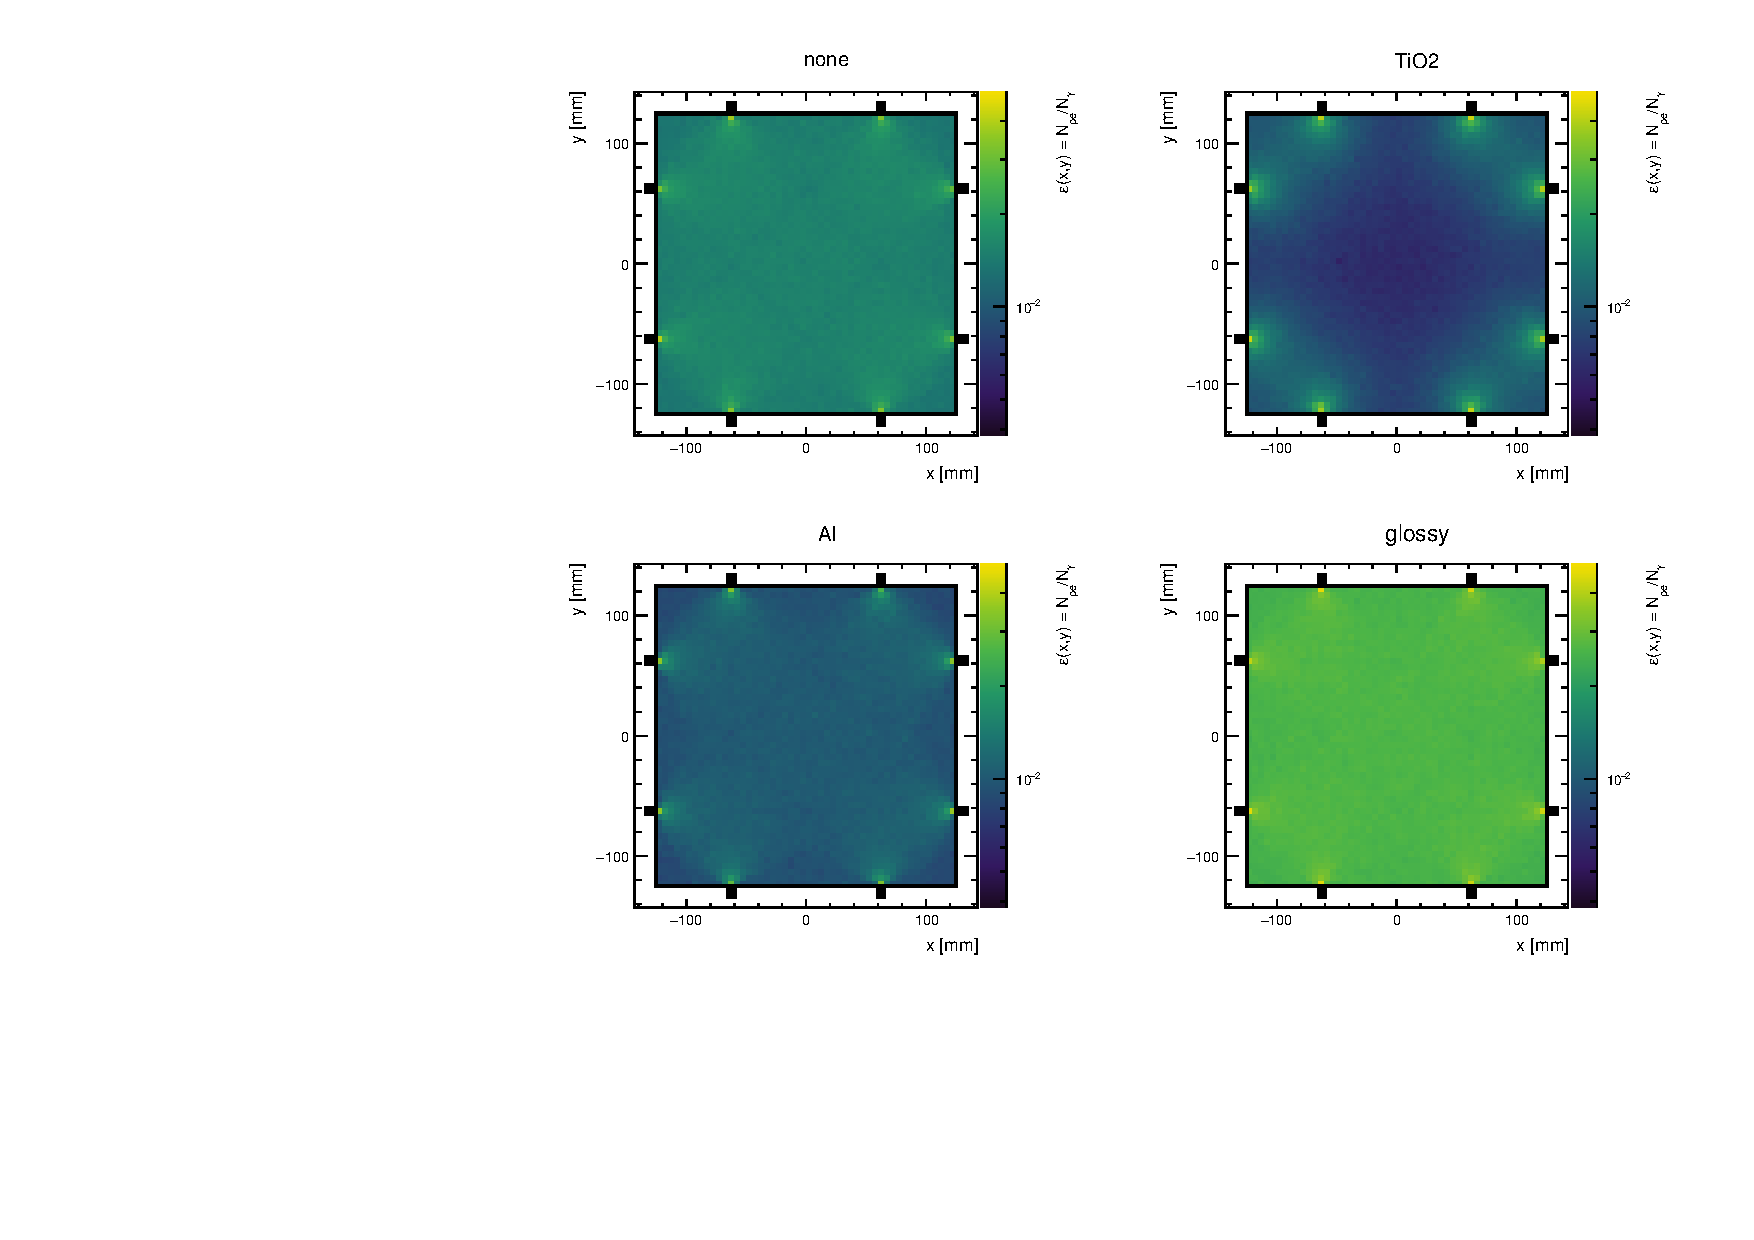
\includegraphics[width=0.82\textwidth]{fig7_whole_maps.pdf}
\caption{Full-plate collection-efficiency maps for config~1, from \num{25000}
whole-plate events per panel ($5\times\SI{5}{\milli\meter}$ cells, logarithmic
colour scale shared by the panels). The bare plate and the specular wrappers are
almost flat; TiO$_2$ is the weakest and the only wrapper with a clear gradient,
dimmest at the centre and brightest toward the edges and corners. The outline is
the \SI{250}{\milli\meter} plate and the squares mark the eight SiPMs.}
\label{fig:maps}
\end{figure}

\begin{table}[htbp]
\centering
\caption{Full-plate position contrast $\ktwo=\eps_{\max}/\eps_{\min}$ over the
\SI{50}{\milli\meter} cells of the whole-plate map. The number in parentheses is
the propagated Poisson uncertainty in the last digits.}
\label{tab:kappa}
\small
\begin{tabular}{@{}lcccc@{}}
\toprule
Wrapper & Config 1 & Config 2 & Config 3 & Config 4 \\
\midrule
Bare    & 1.129(3)  & 1.206(4)  & 1.473(7)  & 1.361(10) \\
TiO$_2$ & 1.902(7)  & 2.543(12) & 8.460(70) & 8.093(81) \\
Al      & 1.186(4)  & 1.329(6)  & 1.792(11) & 1.619(13) \\
Glossy  & 1.069(2)  & 1.119(3)  & 1.273(5)  & 1.161(6)  \\
\bottomrule
\end{tabular}
\end{table}

\subsection{Wavelength and timing}

Figures~\ref{fig:wltime} and~\ref{fig:waveform} show the detected-light
wavelength and arrival-time structure for the glossy whole-plate sample. The
direct-coupled layouts (1--3) detect the blue scintillation spectrum with a
photoelectron-weighted mean of \SIrange{456.7}{457.2}{\nano\meter}. Config~4
is green-shifted to \SI{509.6}{\nano\meter} by the Y-11 absorption and
re-emission, confirming that the WLS process is active and dominates the
config-4 spectrum. In every layout the spectrum reddens with arrival time: the
mean rises from \SI{451}{\nano\meter} ($t<\SI{5}{\nano\second}$) to
\SI{468}{\nano\meter} ($t>\SI{20}{\nano\second}$) for configs~1--3, and from
\SI{499}{\nano\meter} to \SI{511}{\nano\meter} for config~4. The depleted blue
edge of the late light is the signature of self-absorption along the
multi-bounce path and, in config~4, of the wavelength-dependent attenuation of
the fibre.

The timing is equally informative. Configs~1--3 peak at
\SIrange{3.6}{4.1}{\nano\second}, with about \SI{30}{\percent} of the
photoelectrons arriving within \SI{5}{\nano\second} and \SI{60}{\percent}
within \SI{10}{\nano\second}. Config~4 peaks at \SI{9.2}{\nano\second}, with
only \SI{7}{\percent} within \SI{5}{\nano\second} and \SI{33}{\percent} within
\SI{10}{\nano\second}. The late tail ($t>\SI{20}{\nano\second}$) carries
\SIrange{11}{13}{\percent} of the photoelectrons in configs~1--3 but
\SI{25}{\percent} in config~4. The integrated mean yields are \num{520},
\num{275}, \num{141} and \num{68} pe/event for configs~1--4, consistent with
Table~\ref{tab:eff}. The WLS read-out is thus not only less efficient but also
slower, which matters for trigger latency and pile-up.

\begin{figure}[htbp]
\centering
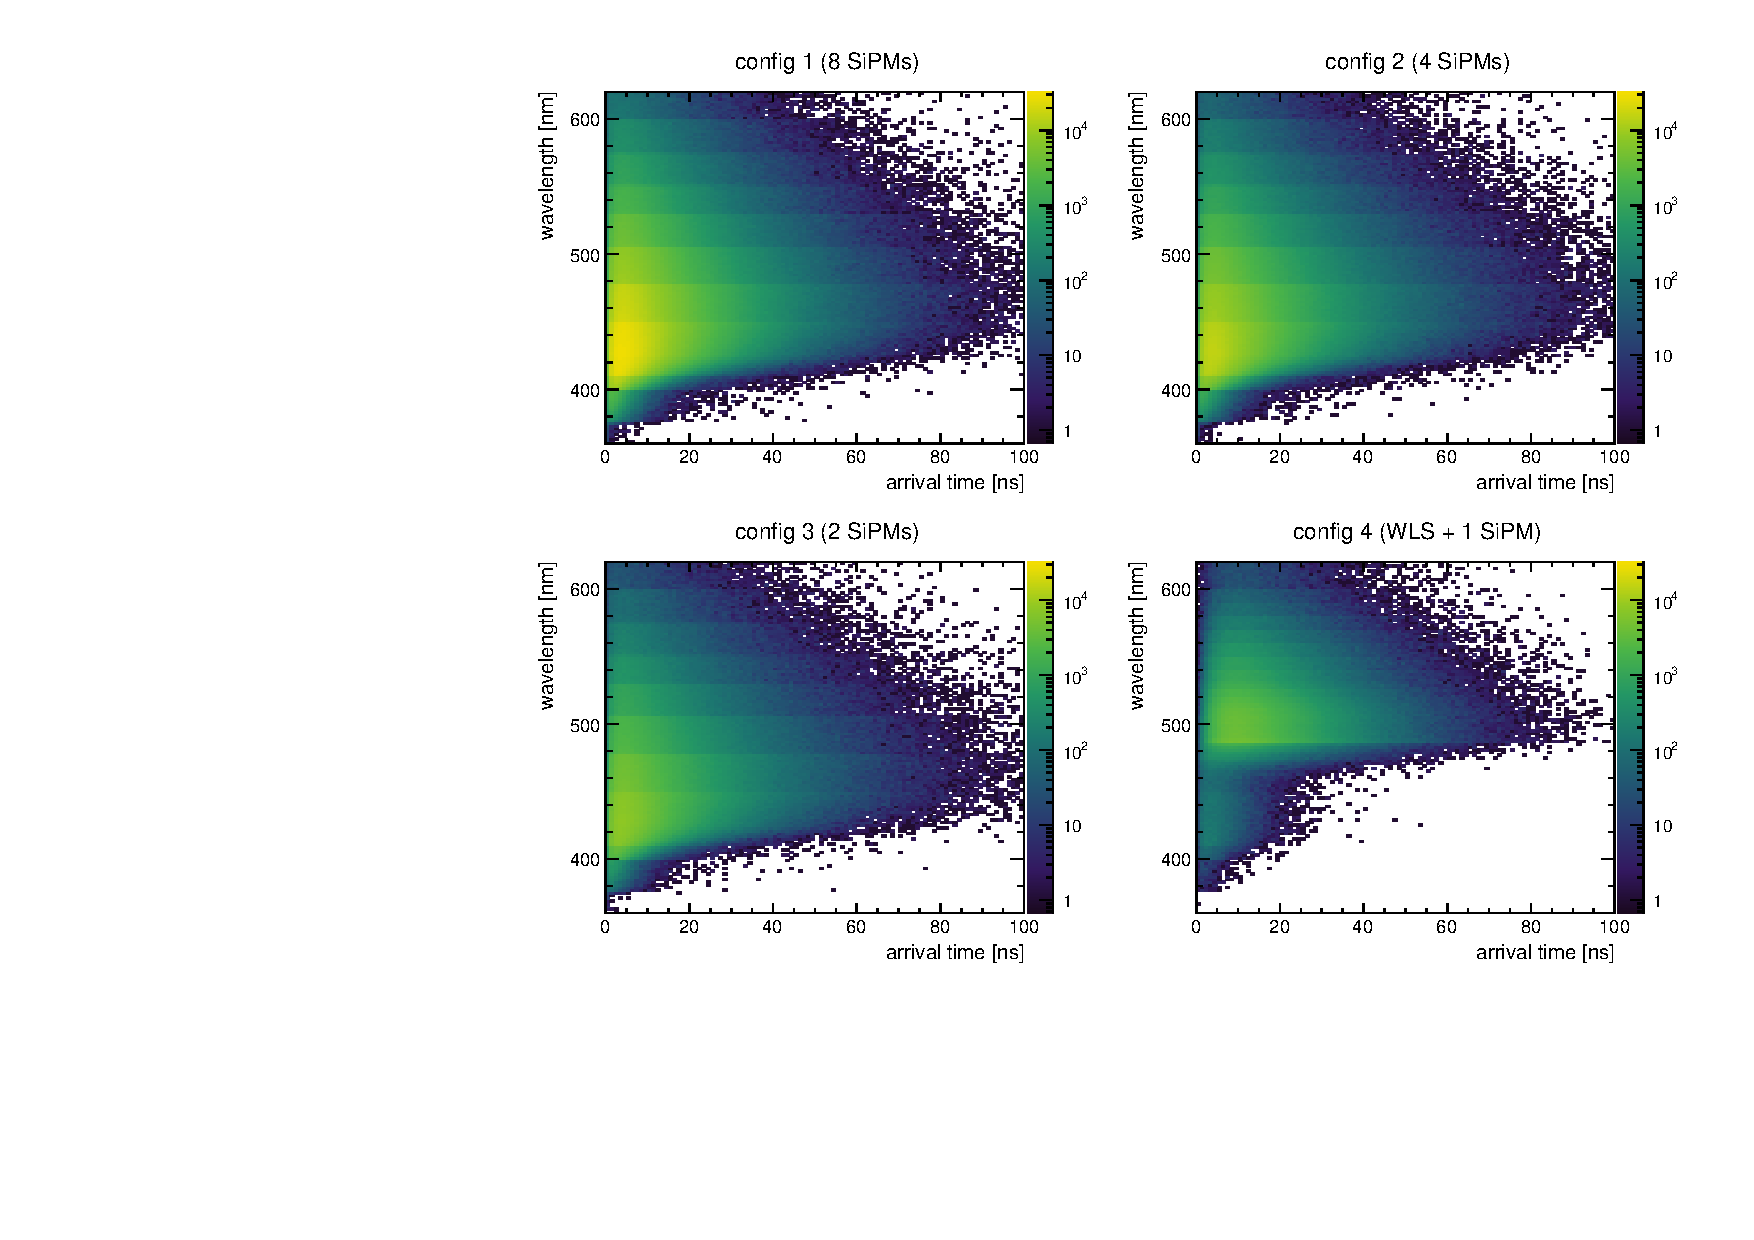
\includegraphics[width=0.95\textwidth]{fig8_wavelength_time.pdf}
\caption{Detected wavelength versus arrival time, one panel per layout (glossy
paper, whole-plate irradiation), on a shared logarithmic colour scale. Layouts
1--3 populate a narrow band around \SI{457}{\nano\meter}; config~4 is
green-shifted by the Y-11 fibres. The mean wavelength increases with arrival
time because the blue edge is preferentially self-absorbed.}
\label{fig:wltime}
\end{figure}

\begin{figure}[htbp]
\centering
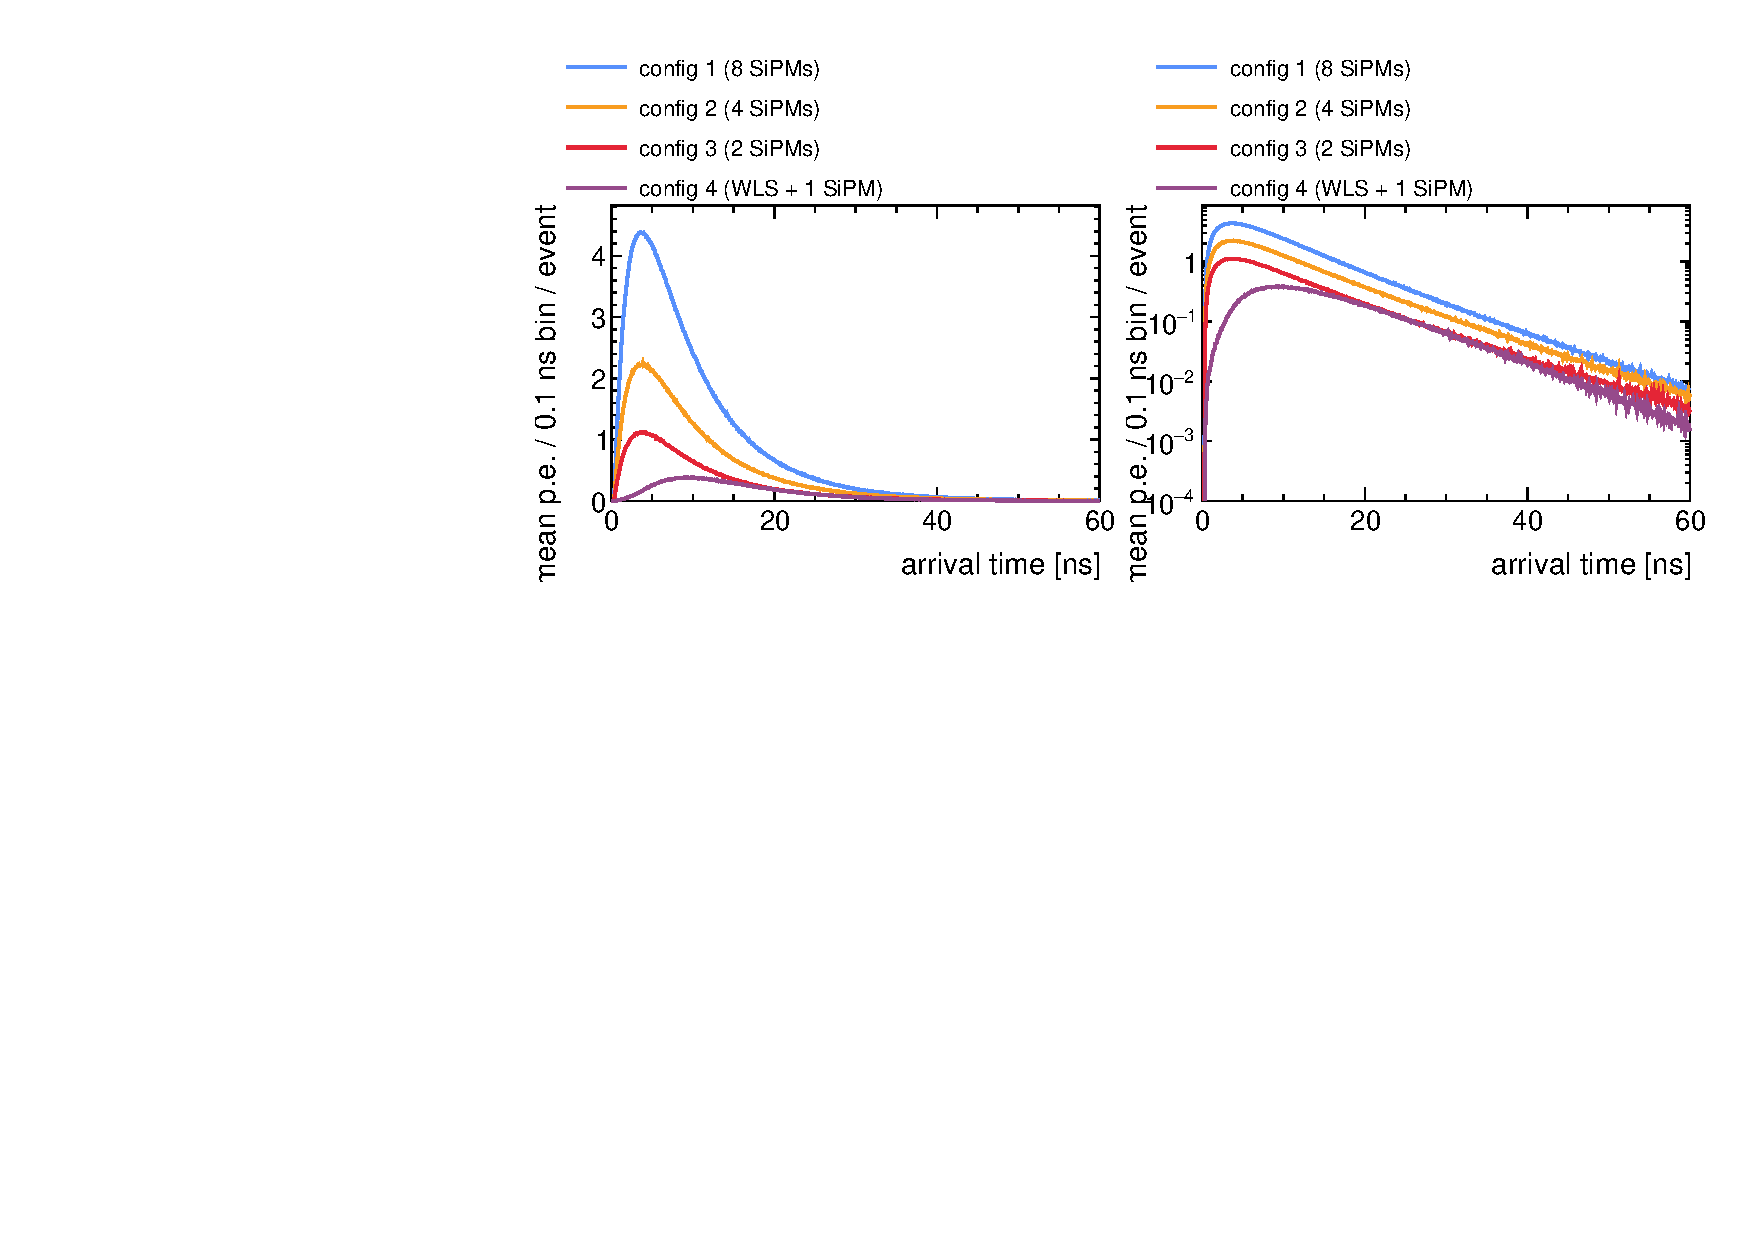
\includegraphics[width=0.95\textwidth]{fig9_waveform.pdf}
\caption{Average arrival-time waveform of the detected photoelectrons, one curve
per layout (glossy paper, whole-plate irradiation). The left panel uses a linear
ordinate and the right a logarithmic one. Configs~1--3 rise within a fraction of
a nanosecond of one another; the WLS layout peaks about \SI{5}{\nano\second}
later and retains a long tail.}
\label{fig:waveform}
\end{figure}

\section{Discussion}
\label{sec:discussion}

\subsection{The bare-plate discrepancy}

The central disagreement with Ref.~\cite{Rao2025} is the bare plate. Their
pulse-height spectra show the bare plate in its black holder as the weakest
configuration, whereas our model gives it the second-highest light yield in the
direct-coupled layouts. The model is not tuned to force agreement. With a true
\SI{1.2}{\milli\meter} air gap, the polished plate is a TIR guide: only the
escape cone ($\theta<\SI{39.3}{\degree}$) is lost, and the trapped light reaches
the edge sensors with little bulk attenuation. The measured suppression
therefore requires a loss channel that is absent from the nominal construction.

Two candidates are physically plausible. The first is optical contact between
the plate and the holder. A real clamped plate touches at scattered high spots;
each contact frustrates TIR and removes trapped light. The second is surface
roughness. A ground or frosted face scatters light out of the TIR cone at every
bounce. Absorption alone is unlikely to explain the suppression: the visible
bulk attenuation length of PVT is metres, so the plate would have to be far
more absorbing than the nominal material to fall below TiO$_2$. Erasing TIR
instead requires a substantially rougher surface than the nominal polished
finish. We did not perform a dedicated roughness scan here. We regard the
air-gap model as the defensible reading of the stated construction (a polished
plate simply set in a holder) and flag the discrepancy rather than tune the
surface to fit the measurement. The practical implication is that the
plate--holder interface, not the wrapper alone, is a first-order design
variable. A controlled experiment that varies the contact area or the surface
finish would test this hypothesis directly.

\subsection{Design guidance}

Several conclusions are robust across layouts. Glossy paper is the brightest and
most uniform wrapper, but it is a model choice as much as a measurement: the
paper is treated as a slightly lossy specular mirror, and real photo paper has a
diffuse component. Aluminium foil with grease is intermediate in the
direct-coupled layouts and weakest in the WLS layout; it is also the most
sensitive to assembly quality, because wrinkles and trapped air reduce its
effective reflectance. TiO$_2$ paint is the weakest and least uniform wrapper in
the direct-coupled layouts; its diffuse recycling helps only when the source is
near a painted edge, and it produces the largest corner-to-centre penalty in the
single-sided layouts. A bare polished plate is an excellent light guide only if
it is genuinely decoupled from its holder; if contact or roughness is
unavoidable, the bare configuration can be the worst choice, as the reference
measurement suggests.

The layout scaling is equally clear. Eight sensors on four faces give the
highest yield; four sensors on four faces halve it; concentrating two sensors on
one face halves it again; and the single-SiPM WLS clamp is about a factor of two
lower still. The WLS layout trades absolute yield for a single read-out channel
and a large effective collection area. Its green-shifted, slower light is a
disadvantage for timing but may be acceptable for a trigger with a loose time
window. A cost-normalized comparison would require the electronics and
dark-count model that this work does not include.

\subsection{Limitations}

The absolute efficiencies are model-dependent. They are fixed by the assumed
light yield, the Birks constant, the PDE curve, the grease coupling and the
tabulated reflectivities. The TiO$_2$ and glossy-paper reflectance curves are
representative fits, not measurements of the actual materials, and the diffuse
lobe of the paint is modelled as ideal Lambertian. The bare plate assumes a
perfect air gap and no contact; this is the largest geometric uncertainty. The
WLS fibre uses a nominal \SI{1.0}{\milli\meter} absorption length at
\SI{430}{\nano\meter}; a systematic band of \SIrange{0.3}{3}{\milli\meter} is
available in the code but not propagated here. The SiPM is modelled as an ideal
photocathode with the datasheet PDE; gain, dark counts, crosstalk,
afterpulsing, electronics thresholds and temperature are not
included~\cite{Anfimov2021}. The primary beam is a monoenergetic
\SI{4}{\giga\electronvolt} muon, not the cosmic spectrum, and the matrix patches
sample only three positions. The statistical uncertainties are quoted, but a
full systematic budget is beyond the scope of this work.

The geometry also contains deliberate simplifications. Configs~3 and~4 are both
placed on the same narrow face, whereas Ref.~\cite{Rao2025} places config~3 on
the top face and config~4 on the left face, i.e.\ on adjacent faces. This
simplification keeps the single-sided layouts directly comparable and opposite
the edge/corner beam patches, but it means the config-3/config-4 comparison is
not an exact reproduction of the reference geometry. The WLS fibre pitch and
convergence length are chosen to fit the \SI{250}{\milli\meter} plate and the
single SiPM; the reference gives less detail on the clamp interior. These choices
affect the absolute config-4 yield, but not the conclusion that the WLS read-out
is slower and less efficient per produced photon.

\section{Conclusion}
\label{sec:conclusion}

We have built a \gfour{} optical model of a polished plastic scintillator read
out by side-mounted SiPMs and used it to study four layouts and four wrapper
treatments at three beam positions and over the whole plate. The model uses the
unified surface model, digitized scintillator and Y-11 tables, a digitized SiPM
PDE and boundary-process photodetection, and it reproduces the measured wrapper
ordering in part: glossy paper is the brightest and most uniform wrapper, and
TiO$_2$ is the weakest and most position-dependent wrapper in the direct-coupled
layouts. The bare plate is the central discrepancy: with a true air gap it is a
near-lossless TIR guide and the second-brightest wrapper, not the weakest. The
measured suppression therefore points to a loss channel at the plate--holder
interface---optical contact or surface roughness---rather than to the wrapper
alone. The WLS layout collects the fewest photoelectrons and is about
\SI{5}{\nano\second} slower, but it uses a single sensor and a large effective
area. The results provide quantitative guidance for wrapper and layout choice
and identify the plate--holder interface as the main ingredient missing from the
present model.

\section*{CRediT authorship contribution statement}
J.~Turko: Conceptualization, Methodology, Software, Validation, Formal analysis,
Investigation, Writing -- original draft.

\section*{Declaration of competing interest}
The author declares no known competing financial interests or personal
relationships that could have appeared to influence this work.

\section*{Data availability}
The simulation code, macros and analysis scripts are available from the author
on reasonable request. The data that support the findings of this study are
available from the corresponding author upon reasonable request.

\section*{Acknowledgements}
The author acknowledges the \gfour{} and ROOT collaborations for their software.

\FloatBarrier
\bibliographystyle{elsarticle-num}
\bibliography{refs}

\end{document}
